\documentclass[12pt]{article}
\usepackage[dvips]{epsfig}
\usepackage{fleqn}
\usepackage{amssymb,amstext}
\usepackage{array}
\usepackage[latin1]{inputenc}
\usepackage{amsmath}
\usepackage[margin=1in]{geometry}
\usepackage{array}
\usepackage{amsmath}
\usepackage{latexsym}
\usepackage{psfrag}
\usepackage{graphicx}
\usepackage{setspace}
\usepackage{caption2}
\usepackage{url}
\usepackage{fancyhdr}
\usepackage{natbib}
\usepackage{cancel}
\usepackage{hyperref}
\usepackage{enumitem}
\usepackage{pdfpages}
\usepackage{indentfirst}
\usepackage{float}

\usepackage{pdflscape}
\usepackage{multirow}
\usepackage{longtable}

\usepackage{xcolor}

\usepackage{subfiles}
 
\usepackage{blindtext}


%\usepackage[utf8]{inputenc}

\hypersetup{
    colorlinks,
    citecolor=black,
    filecolor=[rgb]{0,0.5,0.5},
    linkcolor=black,
    urlcolor=black
}

\renewcommand\listfigurename{}
\renewcommand{\captionlabelfont}{\bf}
\renewcommand{\captionlabeldelim}{.}
\newcommand{\argmax}{\operatornamewithlimits{argmax}}
\renewcommand{\baselinestretch}{2}
\renewcommand\refname{References}
\newcommand\crule[3][black]{\textcolor{#1}{\rule{#2}{#3}}}

\setcounter{secnumdepth}{0}
\makeatletter

%\providecommand*{\input@path}{}
%\g@addto@macro\input@path{{./level1//}{./level1/level2//}{./level2//}}
%\makeatother

%\renewcommand\section{\@startsection {section}{1}{\z@}%
%                                   {-3.5ex \@plus -1ex \@minus -.2ex}%
%                                   {2.3ex \@plus.2ex}%
%                                   {\centering\normalfont\Large\scshape}}
%\renewcommand\subsection{\@startsection {subsection}{1}{\z@}%
%                                   {-3.5ex \@plus -1ex \@minus -.2ex}%
%                                   {2.3ex \@plus.2ex}%
%                                   {\normalfont\bf}}
\renewcommand*\contentsname{}                                   
\pagenumbering{gobble}                                   
\begin{document}
	\begin{center}
	{\bf \Large \textit{Armillaria Gallica} Genome Analysis}\\
	Thomas Bujaki and Kassandra Dickson
	\end{center}

%\section{main}
%All the stuff Thomas did:
%\begin{itemize}
%	\item read depth snapshots - check!
%	\item program to find new significant read depth differences - check!
%	\item average read depth stuff - check!
%	\item total number of aligned reads - check!
%	\item program to take mode of reads - check!
%	\item scaffold graphing program - check!
%	\item read depth differences program - check!
%	\item assemblies
%	\item blasting stuff
%	\item RNA verification
%\end{itemize}
%%%%%%%%%%%%%%%%%%%%%%%%%%%%%%%%%%%
%
%	Read Depth Snapshot
%
%%%%%%%%%%%%%%%%%%%%%%%%%%%%%%%%%%%
\section{Read Depth Snapshots}
\vspace{-0.5cm}
	In order to gain an understanding of how the read depth landscape behaved, we graphed locations which previously Hao Wang had determined to have notably high read depth. There were between 2000 and 4000 regions identified for each of the 15 strains. We graphed each of these regions and all the landscapes appeared to fall into one of four predominant types of high read depth regions: Normal, Rectangular, Right skewed normal, and Left skewed normal.
\begin{figure}[H]
	\begin{centering}
		\resizebox{40mm}{40mm}{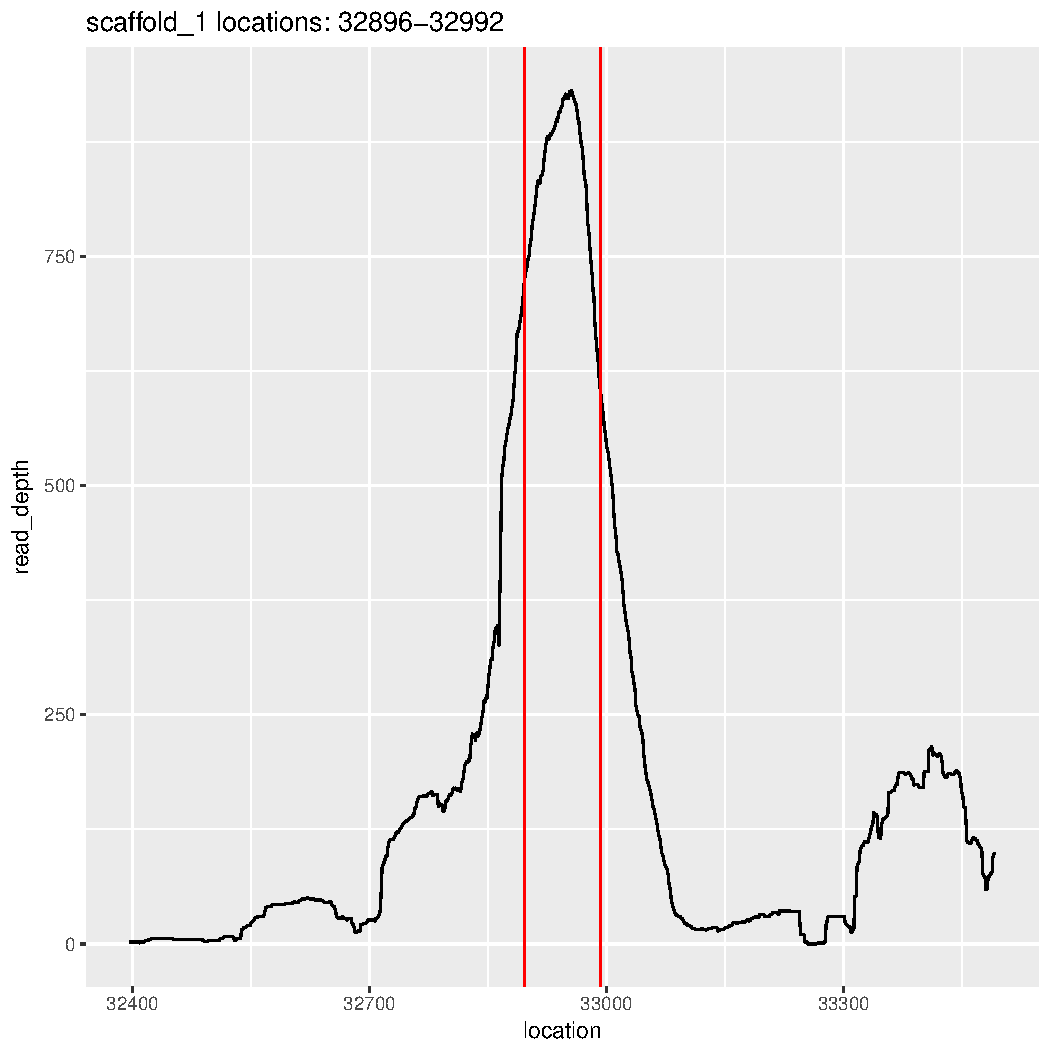
\includegraphics[angle=0,width=1.0\linewidth]{/home/thomas/Directed_Studies_Summer_2019/Armillaria_gallica_gene_analysis_tools/Reporting_documents/Figures/read_depth_snapshot_images/ctj/0_Ar109_read_depth.pdf}}
		\resizebox{40mm}{40mm}{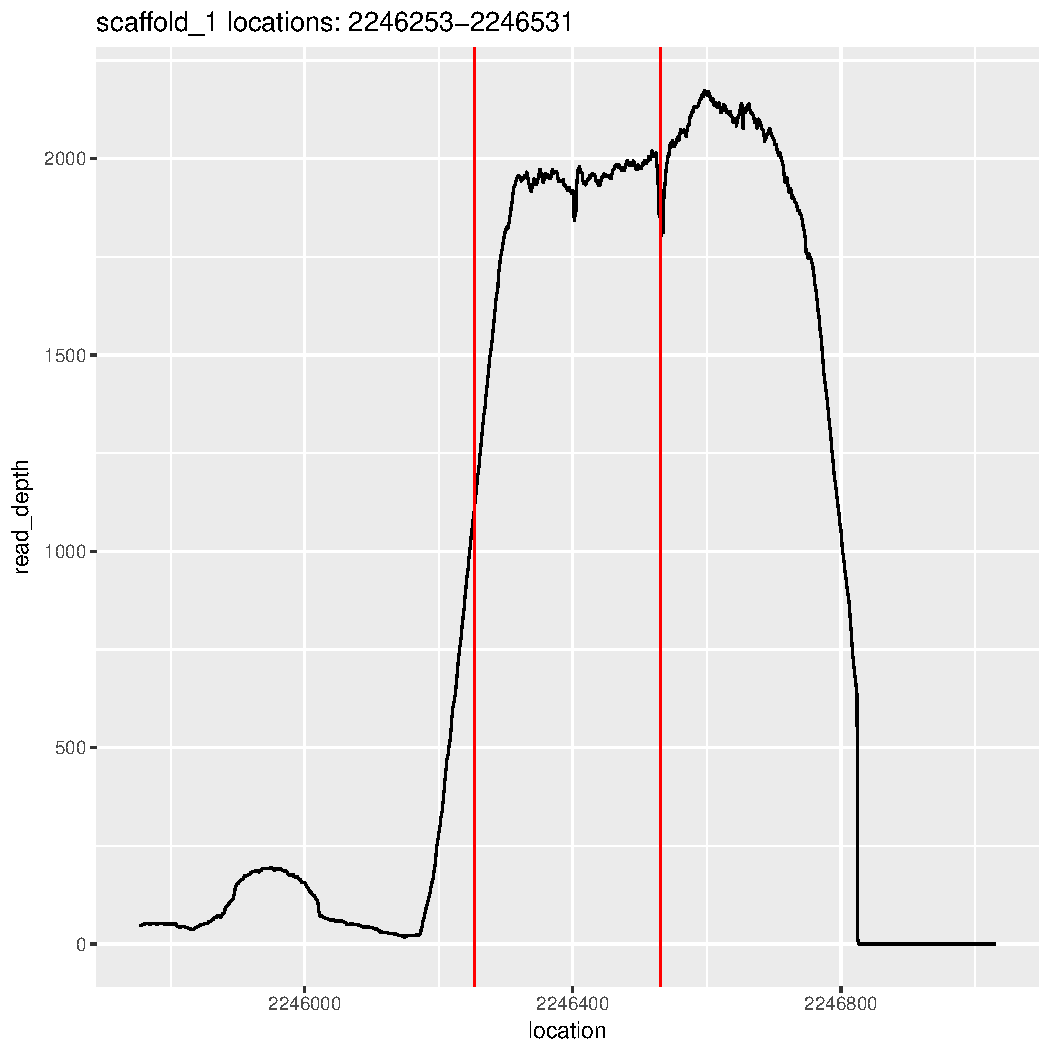
\includegraphics[angle=0,width=1.0\linewidth]{/home/thomas/Directed_Studies_Summer_2019/Armillaria_gallica_gene_analysis_tools/Reporting_documents/Figures/read_depth_snapshot_images/ctj/5_Ar109_read_depth.pdf}}
		\resizebox{40mm}{40mm}{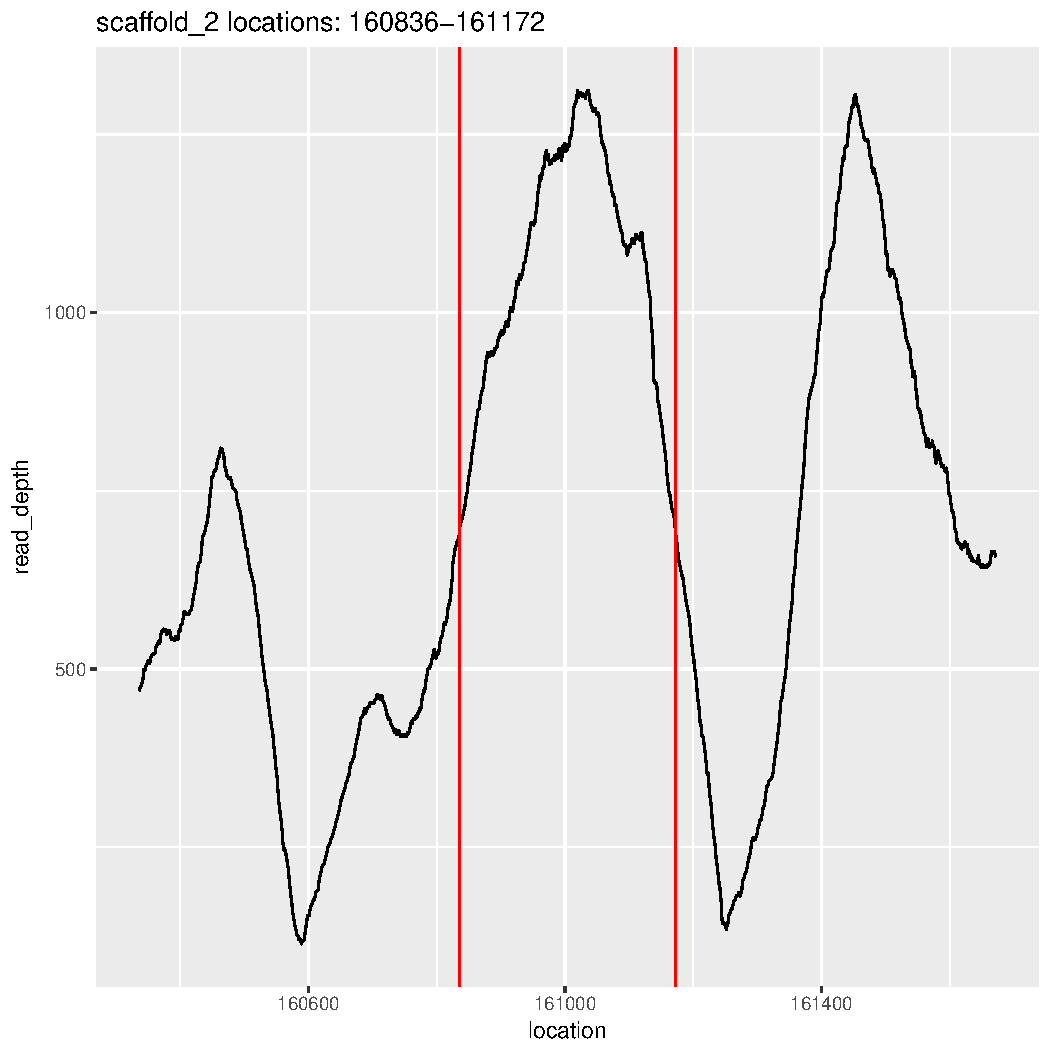
\includegraphics[angle=0,width=1.0\linewidth]{/home/thomas/Directed_Studies_Summer_2019/Armillaria_gallica_gene_analysis_tools/Reporting_documents/Figures/read_depth_snapshot_images/ctj/155_Ar109_read_depth.pdf}}
		\resizebox{40mm}{40mm}{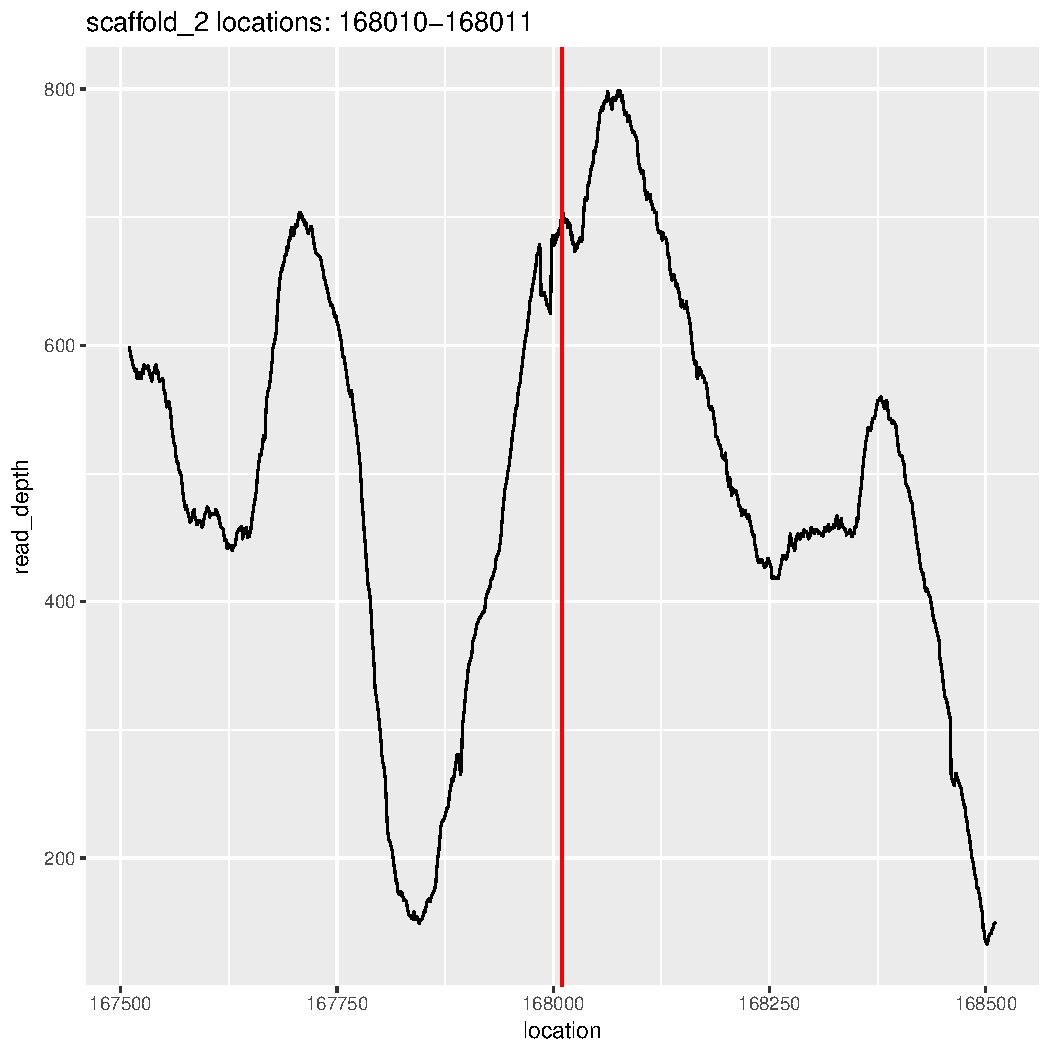
\includegraphics[angle=0,width=1.0\linewidth]{/home/thomas/Directed_Studies_Summer_2019/Armillaria_gallica_gene_analysis_tools/Reporting_documents/Figures/read_depth_snapshot_images/ctj/173_Ar109_read_depth.pdf}}
		\begin{singlespace}
			\vspace{-0.5cm}
			\caption[Examples of the four types of high read depth regions.]{Examples of the four types of high read depth regions (left most) Normal, (left middle) Rectangular, (right middle) Left skewed, (right most)Right skewed}\label{four_rds}
		\end{singlespace}
	\end{centering}
\end{figure}

%%%%%%%%%%%%%%%%%%%%%%%%%%%%%%%%%%%
%
%	Average read depth and total number of reads aligned per scaffold
%
%%%%%%%%%%%%%%%%%%%%%%%%%%%%%%%%%%%
\vspace{-0.5cm}
\section{Average Read Depth}
\vspace{-0.5cm}
	Due to the large quantity of data present in each bam or fastq file we made use of the meta data of the aligned reads in the form of the average number of aligned reads. We calculated the average for each strain and scaffold individually, and also calculated the global average read depth. Locations that did not have any reads aligned to them were not taken into account. The global average read depths are shown in table \ref{globavgrd} and an example of the average read depth per scaffold and the number of aligned reads for each scaffold are graphed in figure \ref{109avgcountgraph}.
\begin{table}[H]
	\begin{center}
		\captionof{table}{Global Average Read Depths and Number of Reads for Each Strain} \label{globavgrd}
		\vspace{0.5cm}
		\scalebox{.7}{
		\begin{tabular}{ |c|c|c| }
			\hline
			Strain & Global Average Read Depth & Total Global Number of Reads \\
			\hline
			Ar73 & 111.0507 & 69955093\\
			\hline
			Ar109 & 117.6863 & 70143802\\
			\hline
			Ar119 & 112.4868 & 70015910\\
			\hline
			Ar142 & 109.3741 & 70068064\\
			\hline
			Ar159 & 104.3773 & 69875550\\
			\hline
			Ar170 & 112.3987 & 70033946\\
			\hline
			Ar174 & 113.4283 & 70022954\\
			\hline
			Ar175 & 73.79959 & 69545937\\
			\hline
			Ar176 & 73.21531 & 69583274\\
			\hline
			Ar179 & 117.2196 & 70061598\\
			\hline
			Ar188 & 63.61699 & 68627951\\
			\hline
			Ar194 & 67.88522 & 69488072\\
			\hline
			Ar196 & 113.9182 & 70027951\\
			\hline
			Ar201 & 68.39596 & 69488227\\
			\hline
			Ar213 & 110.9612 & 69988055\\
			\hline
		\end{tabular}
		}
	\end{center}
\end{table}

\begin{figure}[H]
	\begin{centering}
\vspace{-0.5cm}
		\resizebox{60mm}{60mm}{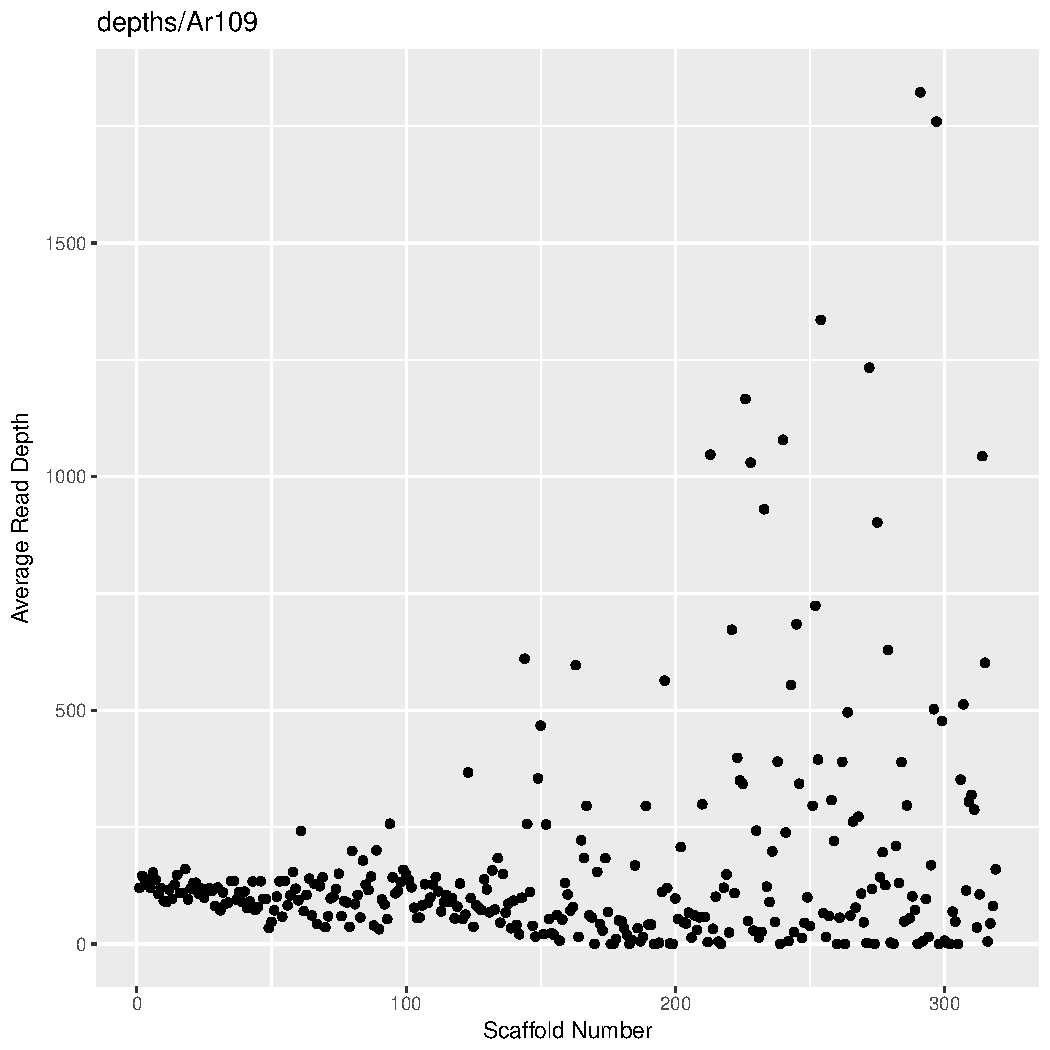
\includegraphics[angle=0,width=1.0\linewidth]{/home/thomas/Directed_Studies_Summer_2019/Armillaria_gallica_gene_analysis_tools/Reporting_documents/Figures/Ar109_collected_no_comma_read_depth.pdf}}
		\resizebox{60mm}{60mm}{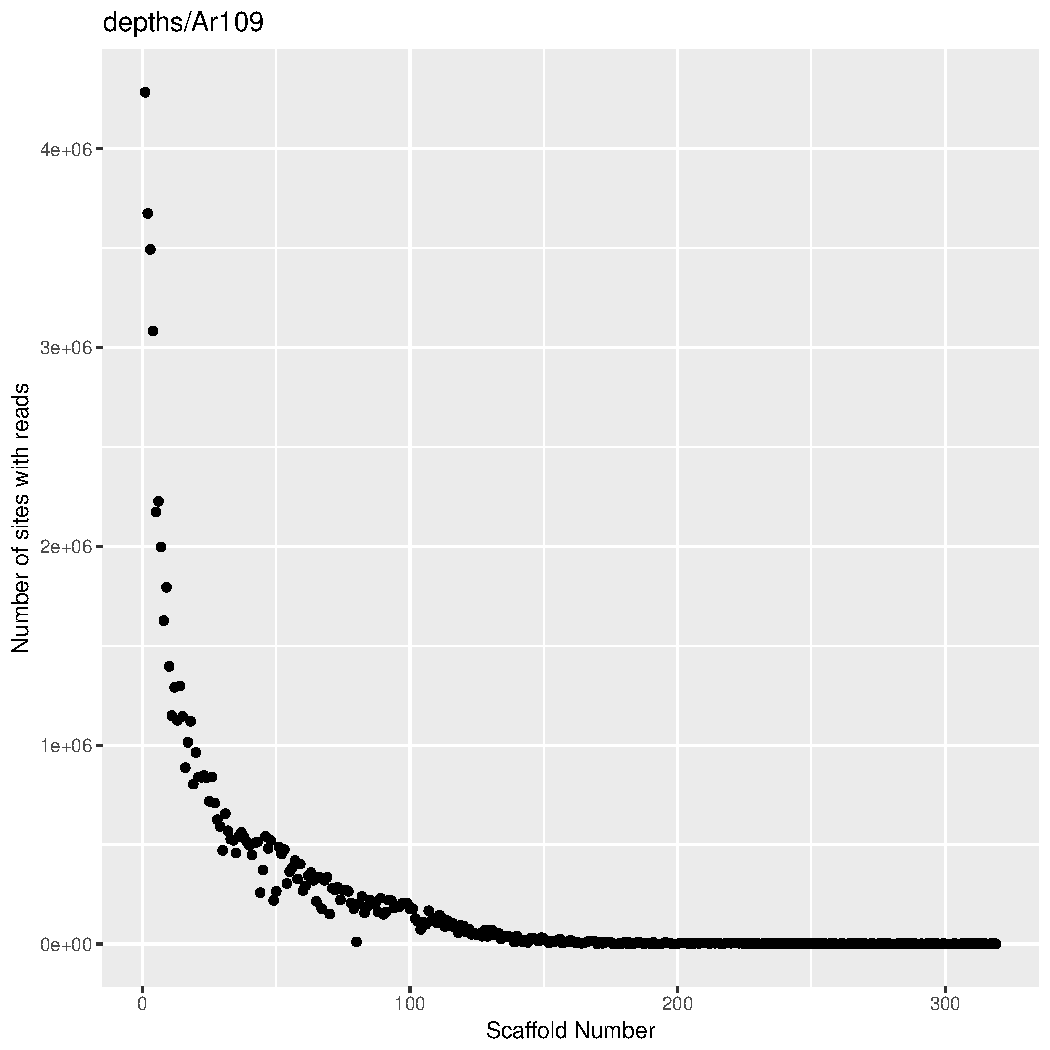
\includegraphics[angle=0,width=1.0\linewidth]{/home/thomas/Directed_Studies_Summer_2019/Armillaria_gallica_gene_analysis_tools/Reporting_documents/Figures/Ar109_collected_no_comma_count.pdf}}\\
		\begin{singlespace}
			\vspace{-0.5cm}
			\caption[Average Read Depth Per scaffold, strain Ar109.]{Average Read Depth Per scaffold and number of aligned reads per scaffold, strain Ar109. (left) average read depth, (right) number of aligned reads.}\label{109avgcountgraph}
		\end{singlespace}
	\end{centering}
\end{figure}

%%%%%%%%%%%%%%%%%%%%%%%%%%%%%%%%%%%
%
%	Identifying Regions of High Read Depth
%
%%%%%%%%%%%%%%%%%%%%%%%%%%%%%%%%%%%
\vspace{-0.5cm}
\section{Identifying Regions of High Read Depth}
\vspace{-0.5cm}
	There were two issues with the methodology Hao used to identify regions of high read depth. The first issue involved cases where the read depth peaked over the search threshold for a small number of locations, this small region would be collected as given the same weight as a larger region regardless of the significance of the short read. This resulted in many locations of apparent significance ranging only a few nucleotides. The second issue was that if a region of significance dipped below the search threshold, then immediately rose back to the level of significance, then a region which should have been contiguous results in two separate regions being identified. We attempted to solve this second issue by creating our own significant read depth search program. This program searched for all locations which were five times the standard deviation above the mean read depth for that scaffold and outputted those regions. The program also allowed for a customisable grace period (set to 10 locations currently) where if the read depth at a location drops below the threshold for less than the grace period then the regions surrounding the dip is treated as contiguous. An example of a read depth snapshot with this issue is shown below in figure \ref{rdsnpstdevgrace}.
\begin{figure}[H]
	\begin{centering}
		\resizebox{50mm}{50mm}{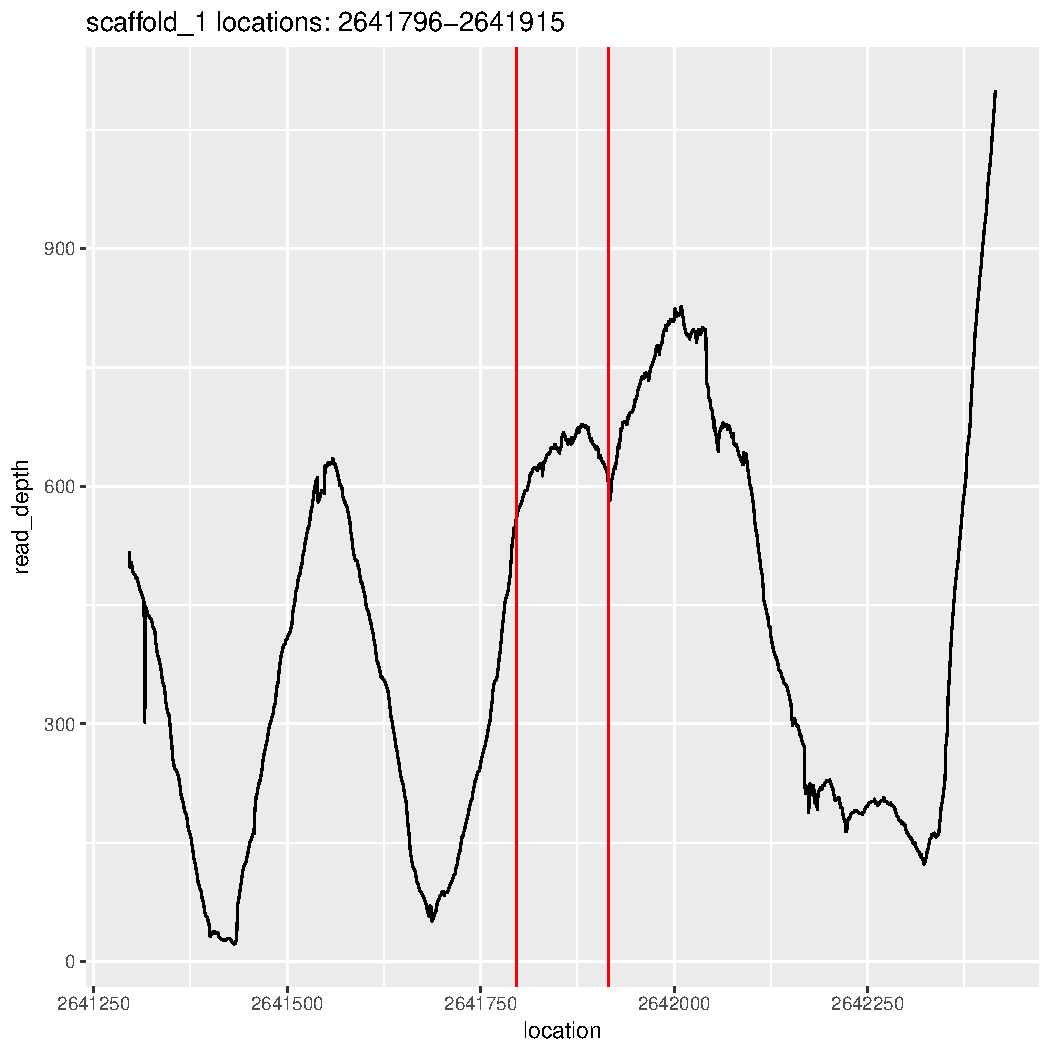
\includegraphics[angle=0,width=1.0\linewidth]{/home/thomas/Directed_Studies_Summer_2019/Armillaria_gallica_gene_analysis_tools/Reporting_documents/Figures/read_depth_snapshot_images/68_Ar109_read_depth.pdf}}
		\resizebox{50mm}{50mm}{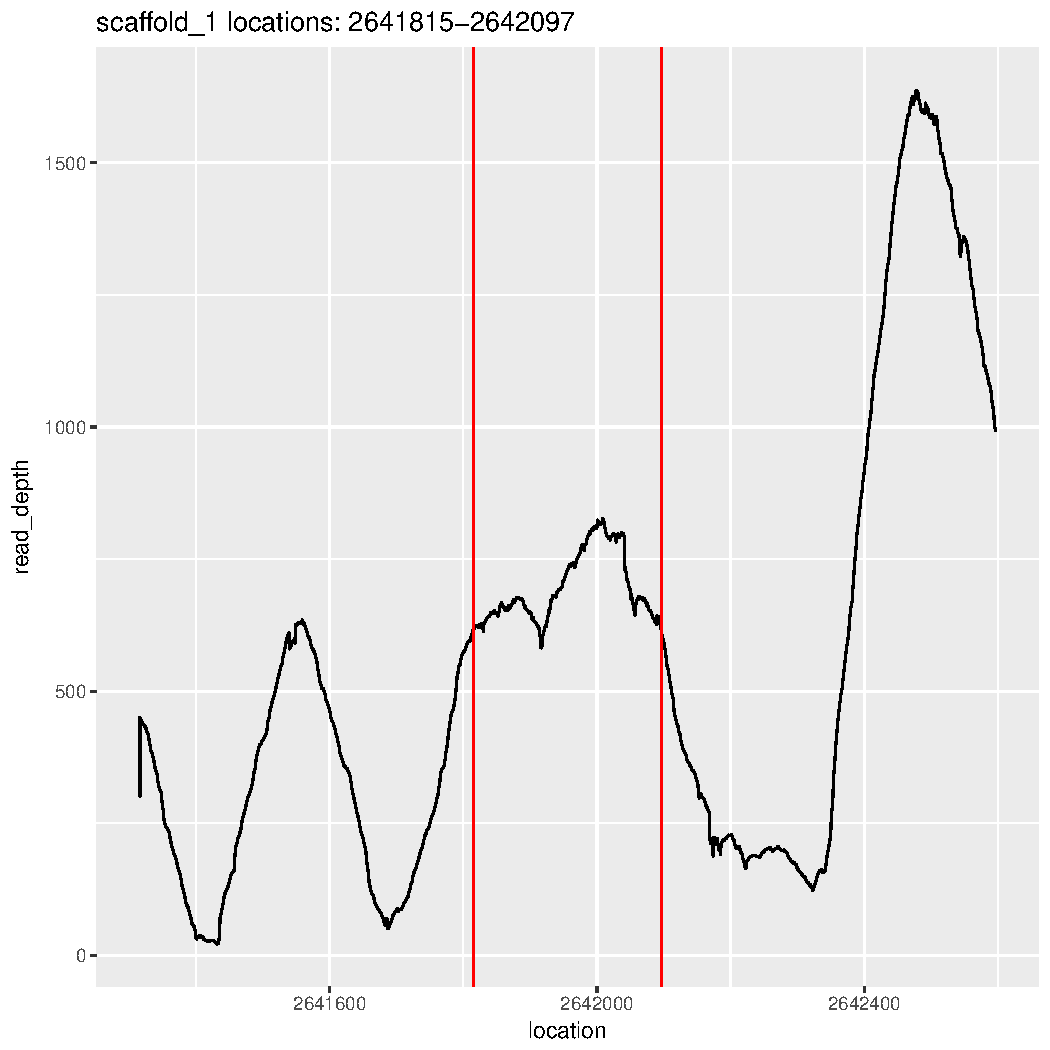
\includegraphics[angle=0,width=1.0\linewidth]{/home/thomas/Directed_Studies_Summer_2019/Armillaria_gallica_gene_analysis_tools/Reporting_documents/Figures/read_depth_snapshot_images/40_Ar109_read_depth.pdf}}\\
		\begin{singlespace}
			\vspace{-0.5cm}
			\caption[Significant Read Depth Identification Differences.]{Significant Read Depth Identification Differences. (left) Hao's method breaks the hill into two parts, (right) method with grace period captures intact read depth hill.}\label{rdsnpstdevgrace}
		\end{singlespace}
	\end{centering}
\end{figure}

%%%%%%%%%%%%%%%%%%%%%%%%%%%%%%%%%%%
%
%	Consensus of Aligned Reads
%
%%%%%%%%%%%%%%%%%%%%%%%%%%%%%%%%%%%
\vspace{-0.5cm}
\section{Consensus of Aligned Reads}
\vspace{-0.5cm}
	Between the identification of locations where there were indels and having many locations of significant read depth we found it necessary to know what the sequence between two locations may be. To do this a series of programs were created which could take in an indexed bam file, a scaffold, a start location, and an end location. This program would then output the mode of all reads aligned within that region. 

%%%%%%%%%%%%%%%%%%%%%%%%%%%%%%%%%%%
%
%	Graphing Read Depth Across Scaffolds
%
%%%%%%%%%%%%%%%%%%%%%%%%%%%%%%%%%%%
\vspace{-0.5cm}
\section{Graphing Read Depth Across Scaffolds}
\vspace{-0.5cm}
	To take a birds eye view of the read depth for each scaffold, we separated each scaffold read depths into their own files and graphed the individual scaffold read depth. The scaffolds vary in size greatly, as can be seen in figure \ref{109avgcountgraph}. Shown below in figure \ref{wholescaffandhisto} are scaffolds 1 and 200 for strain Ar109 and the histograms of the read depths.

\begin{figure}[H]
	\begin{centering}
		\resizebox{110mm}{45mm}{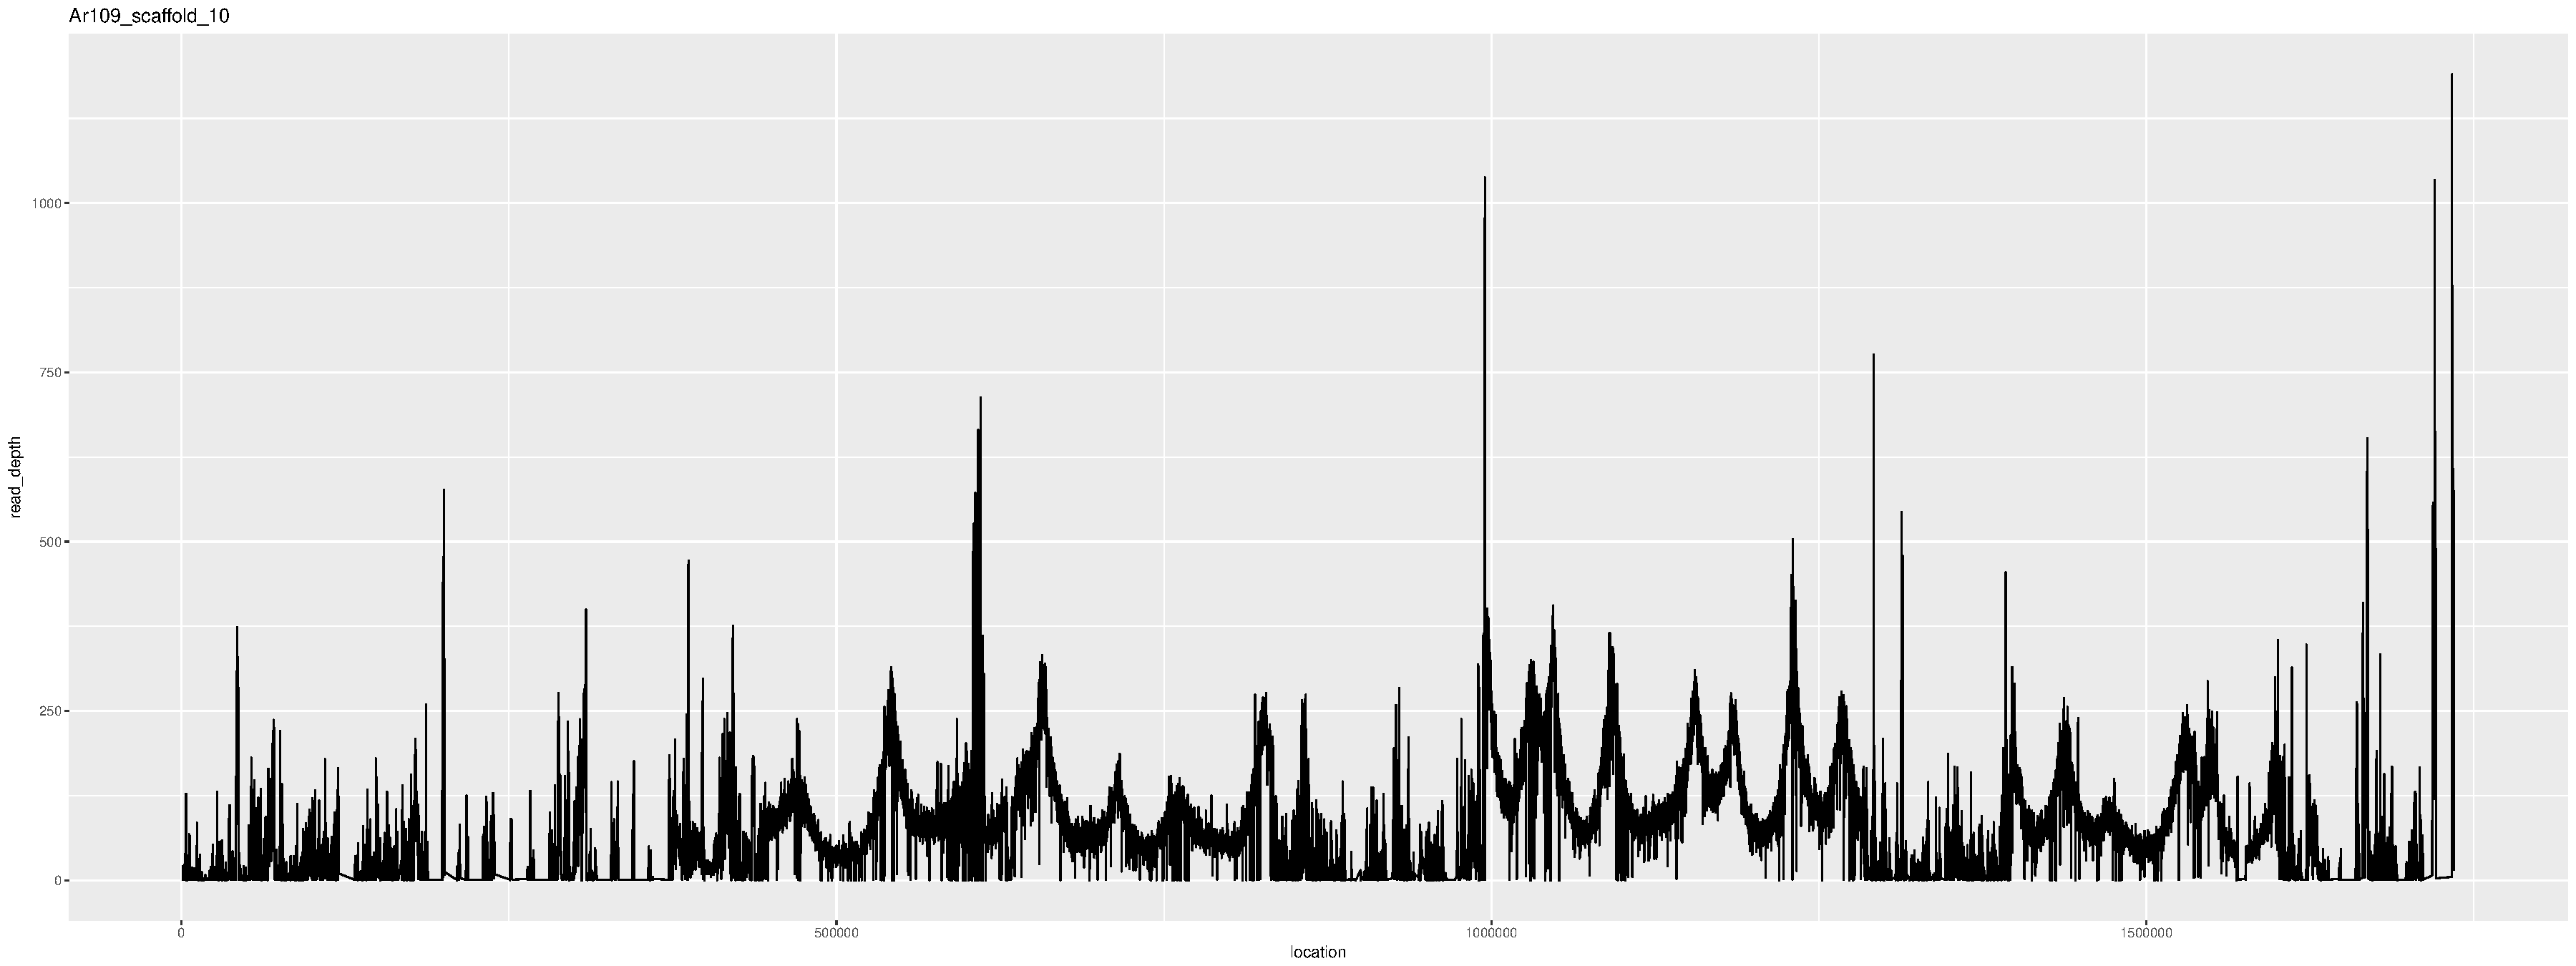
\includegraphics[angle=0,width=1.0\linewidth]{/home/thomas/Directed_Studies_Summer_2019/Armillaria_gallica_gene_analysis_tools/Reporting_documents/Figures/whole_scaffold_images/Ar109_scaffold_10_read_depth.pdf}}
		\resizebox{45mm}{45mm}{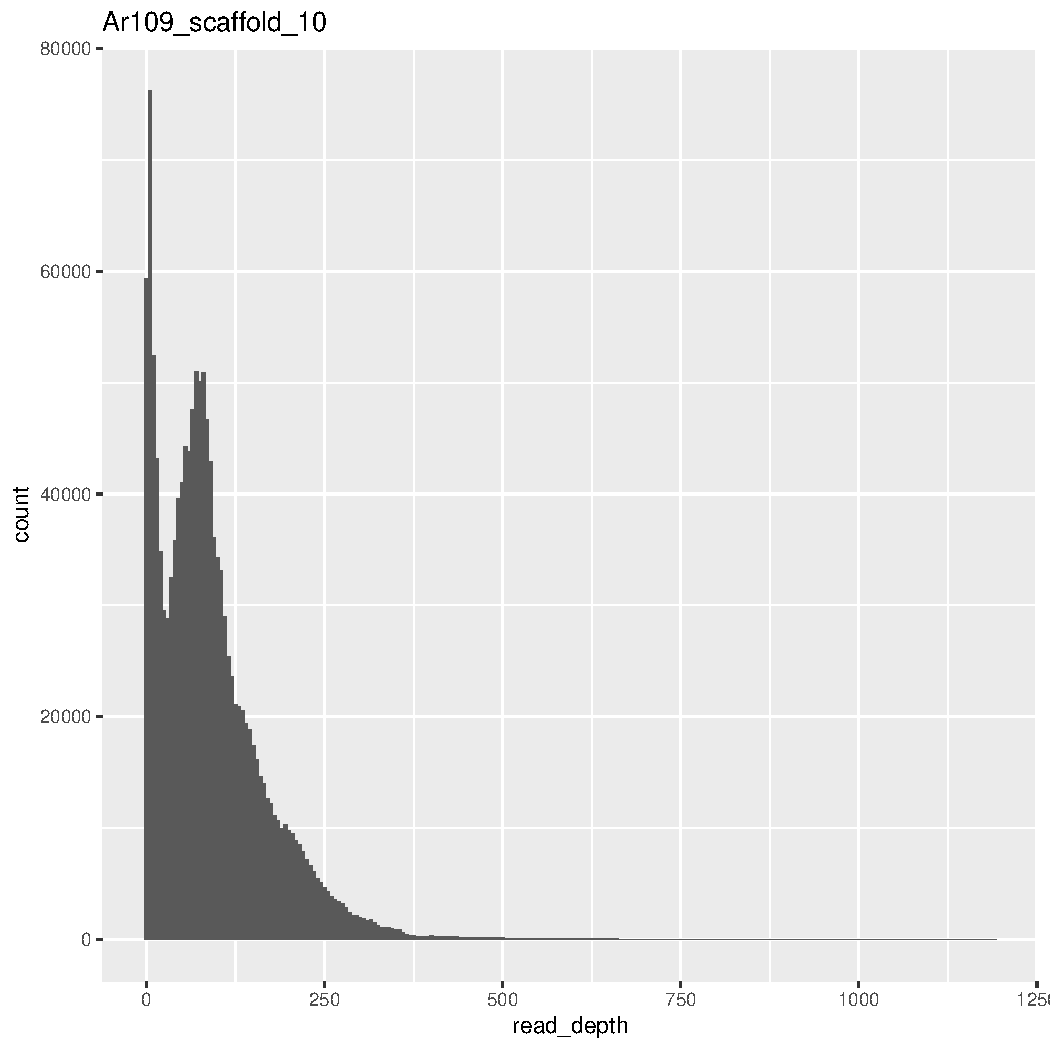
\includegraphics[angle=0,width=1.0\linewidth]{/home/thomas/Directed_Studies_Summer_2019/Armillaria_gallica_gene_analysis_tools/Reporting_documents/Figures/whole_scaffold_images/Ar109_scaffold_10_read_depth_histogram.pdf}}\\
		\resizebox{110mm}{45mm}{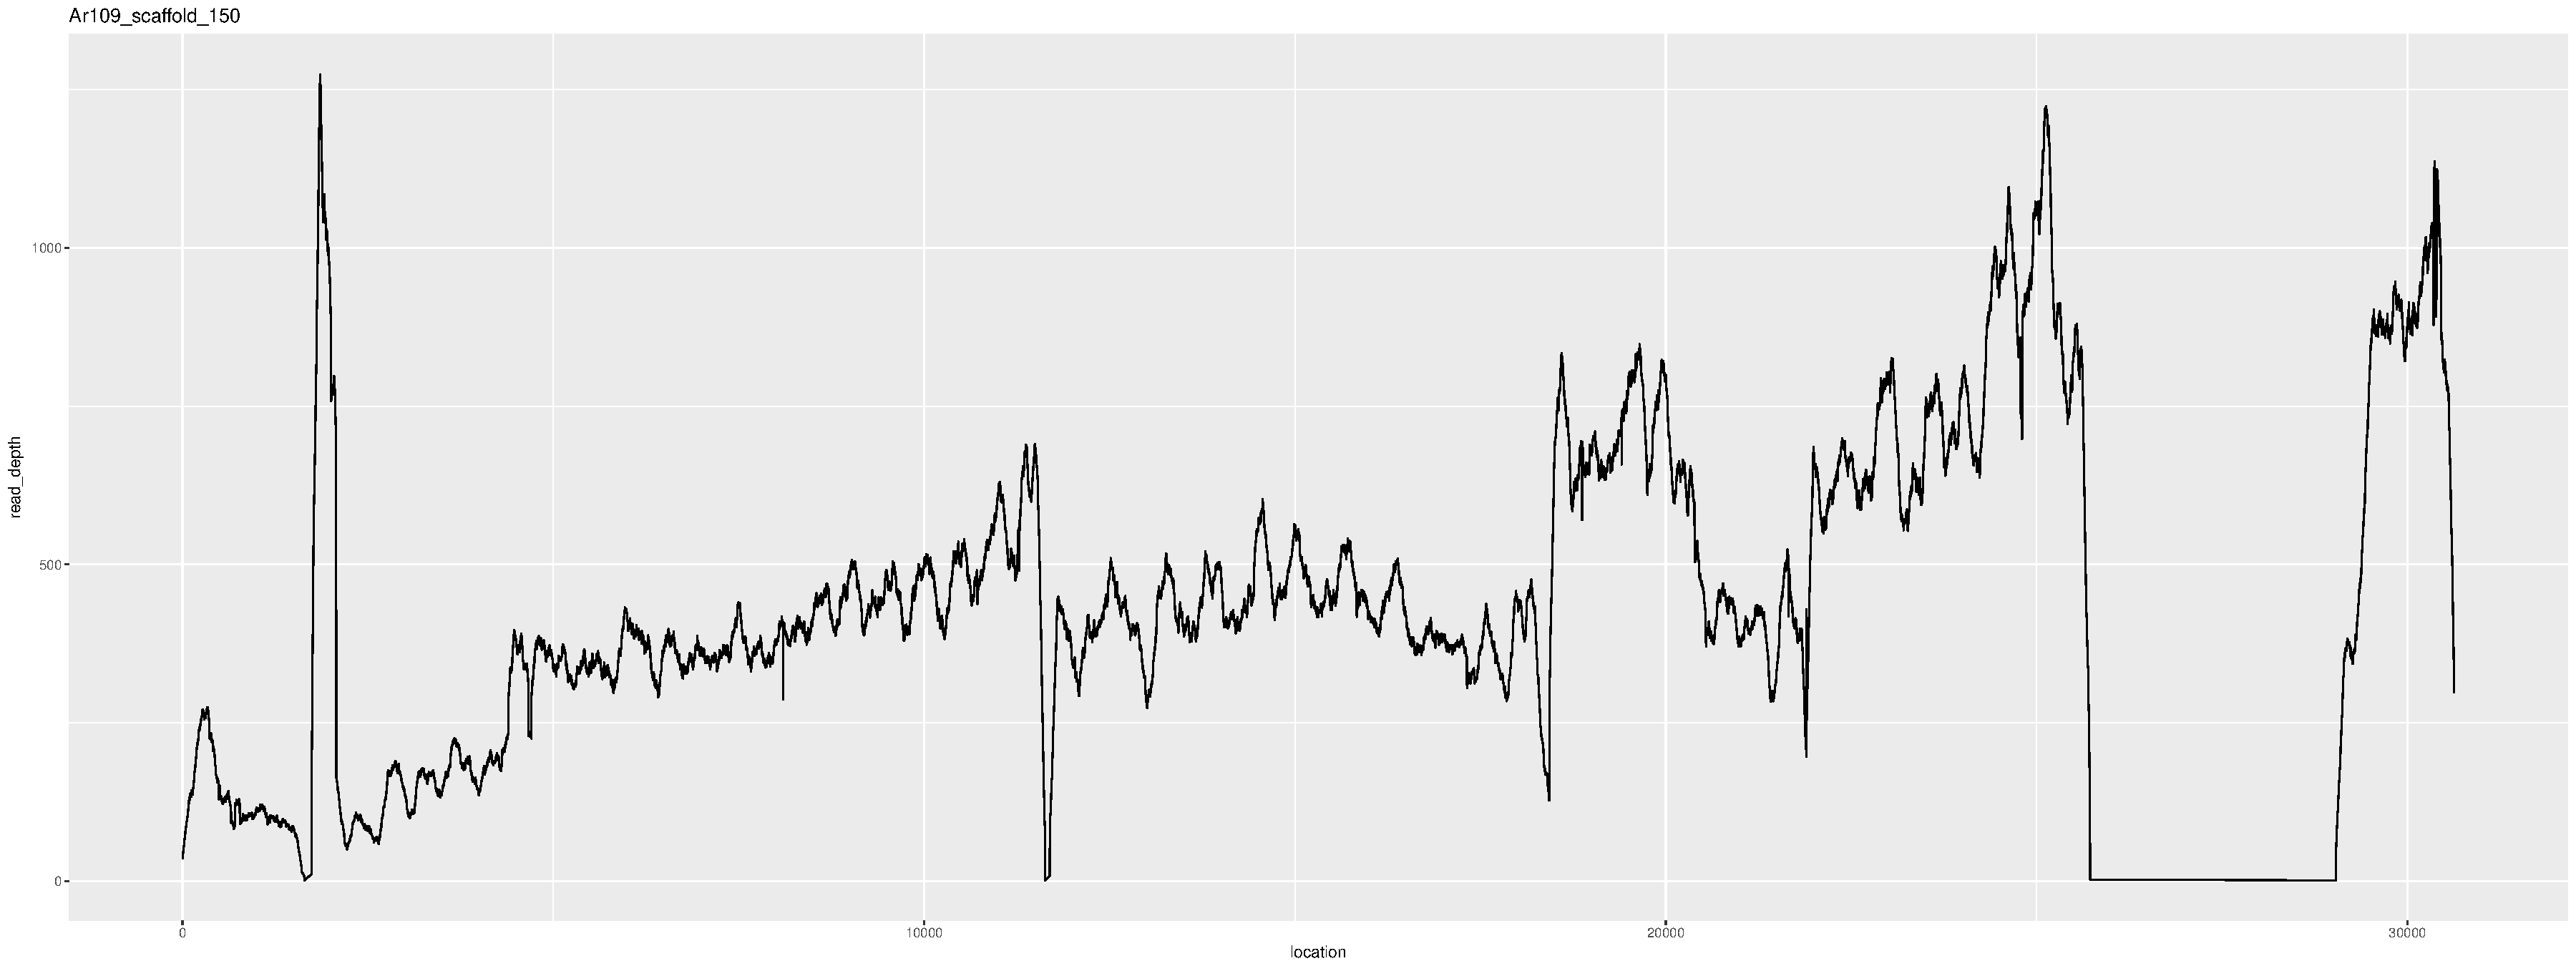
\includegraphics[angle=0,width=1.0\linewidth]{/home/thomas/Directed_Studies_Summer_2019/Armillaria_gallica_gene_analysis_tools/Reporting_documents/Figures/whole_scaffold_images/Ar109_scaffold_150_read_depth.pdf}}
		\resizebox{45mm}{45mm}{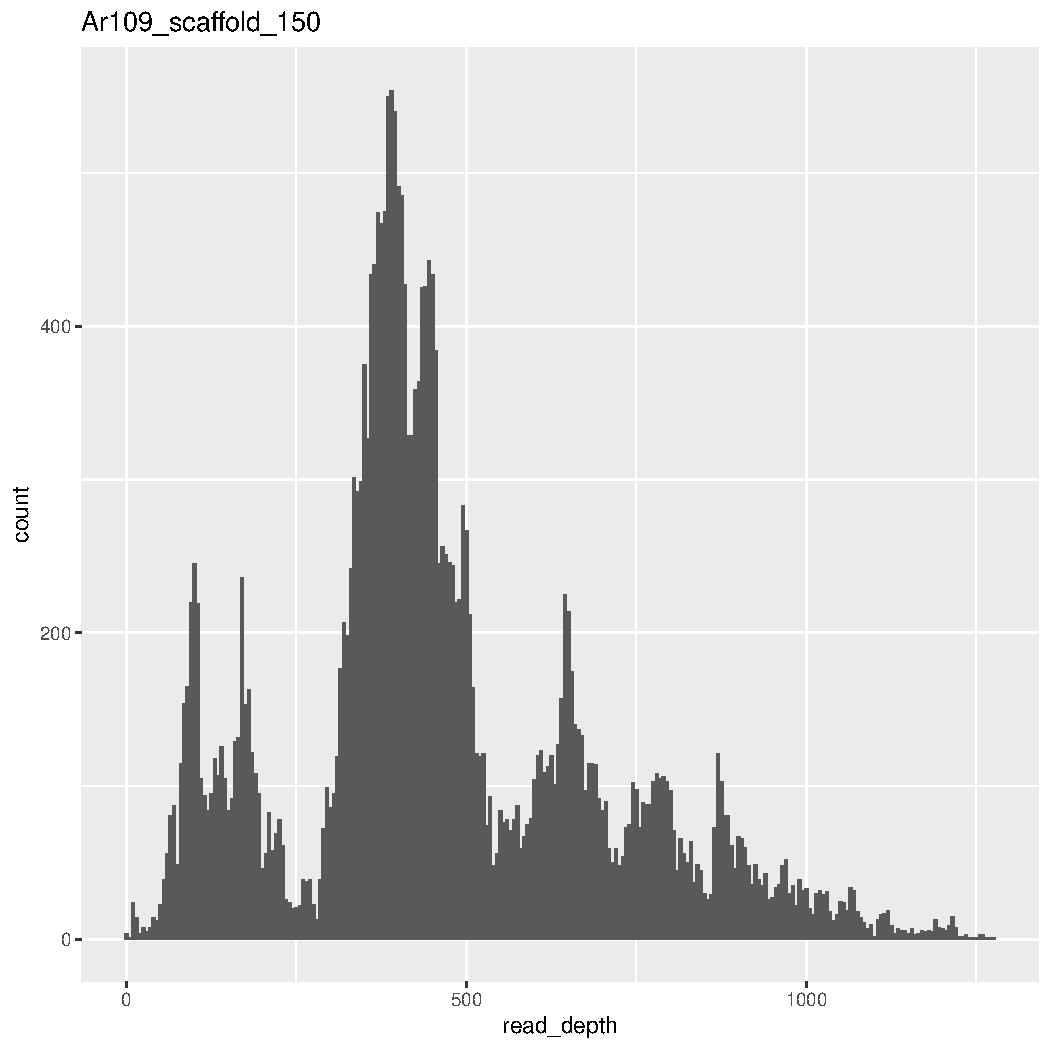
\includegraphics[angle=0,width=1.0\linewidth]{/home/thomas/Directed_Studies_Summer_2019/Armillaria_gallica_gene_analysis_tools/Reporting_documents/Figures/whole_scaffold_images/Ar109_scaffold_150_read_depth_histogram.pdf}}\\
		\begin{singlespace}
			\vspace{-0.5cm}
			\caption[Whole Scaffold Read Depth Graphs.]{Whole Scaffold Read Depth Graphs for strain Ar109. (Top left) Scaffold 10 read depth, (Top right) scaffold 10 histogram, (Bottom left) Scaffold 150 read depth, (Bottom right) scaffold 150 histogram.}\label{wholescaffandhisto}
		\end{singlespace}
	\end{centering}
\end{figure}

%%%%%%%%%%%%%%%%%%%%%%%%%%%%%%%%%%%
%
%	Read Depth Differences Between Strains
%
%%%%%%%%%%%%%%%%%%%%%%%%%%%%%%%%%%%
\vspace{-0.5cm}
\section{Read Depth Differences Between Strains}
\vspace{-0.5cm}
	To compare the read depths between strains we created a program which would iterate over two read depth files and output the differences in read depth at all locations. Due to the similarity of the output from this program to the input used in the program to find significant read depths, we were able to perform the same analysis outlined in the section on identifying regions of high read depth. These sequences could then graphed and searched via blasted.

%%%%%%%%%%%%%%%%%%%%%%%%%%%%%%%%%%%
%
%	Assemblies
%
%%%%%%%%%%%%%%%%%%%%%%%%%%%%%%%%%%%
\vspace{-0.5cm}
\section{Assemblies}
\vspace{-0.5cm}
	The bam files which we were able to work with were created using reference based assembly, but the unaligned reads were stripped from the file. One of the experiments which we wanted to carry out was to create an assembly of the unaligned reads and to see how those 15 assemblies may have compared to each other. In order to gain access to these reads we attempted new reference based assemblies using five of the 15 strains. Although these assemblies have been completed, they have not been analyzed yet due to time constraints.

	We also attempted de novo assemblies of five of the 15 fastq sequences we had. These de novo assemblies were carried out using Velvet and VelvetOptimiser, using default settings. Unfortunately the results from these assemblies were of low quality. The largest contig was roughly 5000 bases and the total number of contigs was over 150,000. In the future we will attempt to determine why these de novo assemblies turned out so poorly. We also attempted to combine some of the sequences into a single large fastq file. We are in the process of creating a de novo assembly of this large file.

%%%%%%%%%%%%%%%%%%%%%%%%%%%%%%%%%%%
%
%	Sequence Identification With Blastn
%
%%%%%%%%%%%%%%%%%%%%%%%%%%%%%%%%%%%
\vspace{-0.5cm}
\section{Sequence Identification With Blastn}
\vspace{-0.5cm}
	Making use of the identified regions of high read depth and the program which can extract sequences from bam files, we were able to use blastn to attempt to determine the function of the different notable sequences. Due to the high number of sequences we were only able to search a small fraction of the total, and the results from those searches were inconclusive. Nearly all of the sequences searched had no hits and the few that did were mainly mRNA sequences. We determined that there is a method to carry out multiple blastn searches quickly, although we have not yet been able to make the program needed for this to function. When we can get this method working we will be able to carry out an automated blast search of any sequence we find interesting.   

%%%%%%%%%%%%%%%%%%%%%%%%%%%%%%%%%%%
%
%	Sequence Identification With Blastn
%
%%%%%%%%%%%%%%%%%%%%%%%%%%%%%%%%%%%
\vspace{-0.5cm}
\section{RNA Verification of Blast Method}
\vspace{-0.5cm}
	Due to the low number of significant blast results, we attempted to verify this method of sequence identification by attempting to find a sequence which we know to be present in \textit{Armillaria Gallica}. Specifically we obtained a partial 18S rRNA sequence for the fungus \textit{Aspergillus niger} that was roughly 1700 nucleotides long, and blasted that sequence against the reference genome for \textit{Armillaria Gallica} on the Joint Genome Institute Fungal Genomics Resource website. This blast returned a hit for a small region on scaffold 10 (scaffold 10:994951-995150), although this region was only 199 nucleotides in length. When we searched for this region in our scaffold snapshot graphs we were able to find that it was identified as a region of notable read depth by our system. The read depth snapshot for this range is shown in figure \ref{rdsnp18Srrna}. The total ribosomal DNA for \textit{Armillaria Gallica} should be larger than 10kb and the 18S subunit should be larger than 3kb. We did complete a search on ncbi for the entire ribosomal DNA sequence but we could only find partial 28S sequences and partial 18S/28S sequences. When blasting the partial 18S/28S sequence against the reference we found no matches. A portion of partial 28S subunit could be verified using the same method used for the 18S subunit. We suspect that the reference file does not include the whole ribosomal DNA sequence and it may be that the ribosomal sequences present in the 15 strains of \textit{Armillaria Gallica} are contained in the unaligned reads following reference based assembly. 
      \begin{figure}[H]
	\begin{centering}
\resizebox{50mm}{50mm}{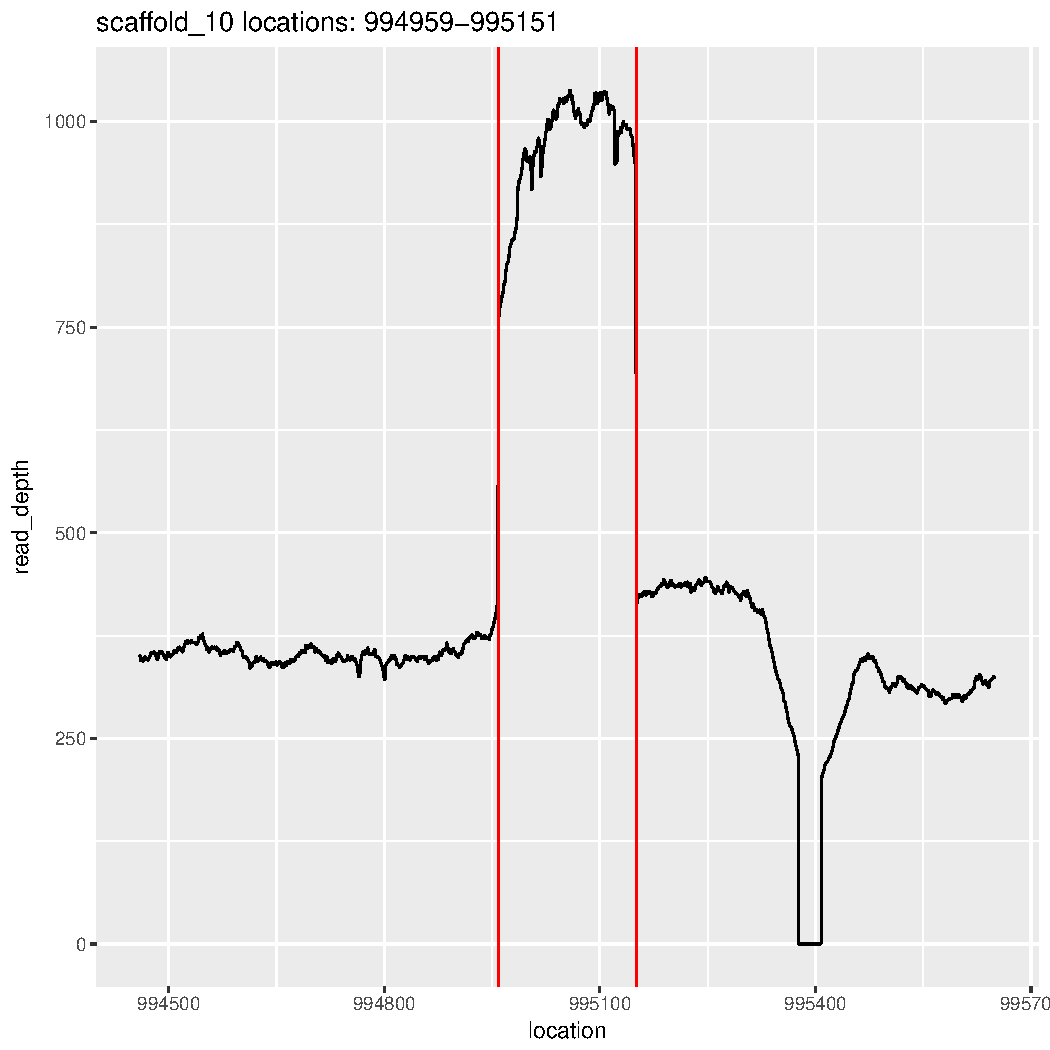
\includegraphics[angle=0,width=1.0\linewidth]{/home/thomas/Directed_Studies_Summer_2019/Armillaria_gallica_gene_analysis_tools/Reporting_documents/Figures/read_depth_snapshot_images/433_Ar109_read_depth.pdf}}
 		\begin{singlespace}
			\vspace{-0.5cm}
			\caption[Read Depth for Partial 18S Sequence.]{Read Depth for Partial 18S Sequence.}\label{rdsnp18Srrna}
		\end{singlespace}
	\end{centering}
\end{figure}
%%%%%%%%%%%%%%%%%%%%%%%%%%%%%%%%%%%
%
%	Indel Analysis
%
%%%%%%%%%%%%%%%%%%%%%%%%%%%%%%%%%%%
\vspace{-1cm}
\section{Indel Analysis}
\vspace{-0.5cm}
In order to start exploring InDels, a mpileup file was made for all 15 strains. This was done by using the command in samtools \textit{mpileup}. A pileup file is a text-based format for summarizing the calls of aligned reads to the reference sequence. This format also allows for visual displays of SNP/indel calling and alignments. Once, a pileup file was produced. It is at this point, where output tags were included into the data. These output tags will indicate the read depth, quality score and also anything else that may be of use for analysis.  A package called \textit{BCFtools} was implemented. BCFtools is a set of utilities that manipulate variant calls in the variant call format (vcf) as well as its binary counterpart (bcf). The pileup file was indexed using the command \textit{bcftools index}. This creates an index of the sequence from the pileup file. After this is done, we use the command \textit{bcftools call}, which is the variant calling. This will call the indels in this case and produce a .vcf and a .bcf file which show the indels and their locations. The script which does this process is called \textit{ctq\_reads\_find\_indels.sh}. 

It appears at first glance that there was many indels detected that were the same throughout the strains as seen in \ref{tab:sum_indel}. The summary table only shows the first three indels found within each strain, however throughout the data, this is a repeated pattern. 

\begin{table}[H]
	\begin{center}
		\vspace{-1cm}
		\begin{singlespace}
			\captionof{table}[Summary Indel Table]{A summary table of the first three indels found in each of the strains which includes the scaffold number, the location at which the indel is found, the number of reads that support that indel, and the raw read depth\\} \label{tab:sum_indel}
			\scalebox{.7}{
				\begin{tabular}{ |c|c|c|c|c|c|c| } 
					\hline
					Strain No. & Scaffold No. & Location & No. of Reads Supporting & Raw Read Depth \\
					\hline
					\multirow{3}{4em}{Ar73} & 1 & 7762 &54 & 156\\
					&1 & 10784 & 34 & 148\\
					&1 & 12340 & 37 & 123\\
					\hline
					\multirow{3}{4em}{Ar109} & 1 & 7762 & 56 & 163\\
					& 1 & 10784 & 68 & 175 \\
					& 1 & 16154 & 7 & 176 \\
					\hline
					\multirow{3}{4em}{Ar119} & 1 & 7762 & 62 & 163 \\
					& 1 & 10784 & 57 & 140 \\
					& 1 & 16154 & 4 & 167 \\
					\hline
					\multirow{3}{4em}{Ar142} & 1 & 7762 & 63 & 189 \\
					& 1 & 10784 & 55 & 186 \\
					& 1 & 16154 & 5 & 125 \\
					\hline
					\multirow{3}{4em}{Ar159} & 1 & 7762 & 41 & 116 \\ 
					& 1 & 10784 & 28 & 100  \\ 
					& 1 & 16154 & 3 & 85 \\ 
					\hline
					\multirow{3}{4em}{Ar170} & 1 & 7762 & 73 & 222 \\ 
					& 1 & 10784 & 61 & 194  \\ 
					& 1 & 12340 & 72 & 193 \\ 
					\hline
					\multirow{3}{4em}{Ar174} & 1 & 7762 & 63 & 201 \\ 
					& 1 & 9593 & 72 & 218  \\ 
					& 1 & 10784 & 45 & 184 \\ 
					\hline
					\multirow{3}{4em}{Ar175} & 1 & 7762 & 47 & 141 \\ 
					& 1 & 10784 & 28 & 108  \\ 
					& 1 & 12340 & 35 & 102 \\ 
					\hline
					\multirow{3}{4em}{Ar176} & 1 & 7762 & 39 & 141 \\ 
					& 1 & 9593 & 43 & 129  \\ 
					& 1 & 10784 & 33 & 115 \\ 
					\hline
					\multirow{3}{4em}{Ar179} & 1 & 7762 & 63 & 193 \\ 
					& 1 & 9593 & 64 & 205  \\ 
					& 1 & 10784 & 50 & 195 \\ 
					\hline
					\multirow{3}{4em}{Ar188} & 1 & 7762 & 17 & 62 \\ 
					& 1 & 10784 & 11 & 47  \\ 
					& 1 & 12340 & 24 & 54 \\ 
					\hline
					\multirow{3}{4em}{Ar194} & 1 & 7762 & 35 & 133 \\ 
					& 1 & 10784 & 32 & 105  \\ 
					& 1 & 12340 & 35 & 110 \\ 
					\hline
					\multirow{3}{4em}{Ar196} & 1 & 7762 & 72 & 224 \\ 
					& 1 & 10784 & 53 & 169  \\ 
					& 1 & 12340 & 72 & 192 \\ 
					\hline
					\multirow{3}{4em}{Ar201} & 1 & 7762 & 38 & 110 \\ 
					& 1 & 10784 & 44 & 116  \\ 
					& 1 & 12340 & 50 & 102 \\ 
					\hline
					\multirow{3}{4em}{Ar213} & 1 & 7762 & 76 & 220 \\ 
					& 1 & 9593 & 63 & 196  \\ 
					& 1 & 10784 & 48 & 188 \\ 
					\hline
				\end{tabular}
			}
		\end{singlespace}
	\end{center}
\end{table}

\subsection{Read Depth of Indels}

Read depth or sequence depth was one of the output tags that we added to the pileup file previously. Read depth was important in this analysis thus, we decided to explore them as part of the indel analysis. Since, it was already one of the output tags we previously added, it was a very simple as to extract the datapoint with the corresponding scaffold and location. These were plotted as to see which regions or scaffolds had the highest read depth and to see if the read depth overall was appropriate for further directions.

It was shown that there was good read depth generally throughout the scaffolds. The larger the scaffold, the more indels occurred however, the read depth still holds to be good. 

\begin{figure}[H]
	\begin{centering}
		%\vspace{1.5cm}
		\resizebox{50mm}{50mm}{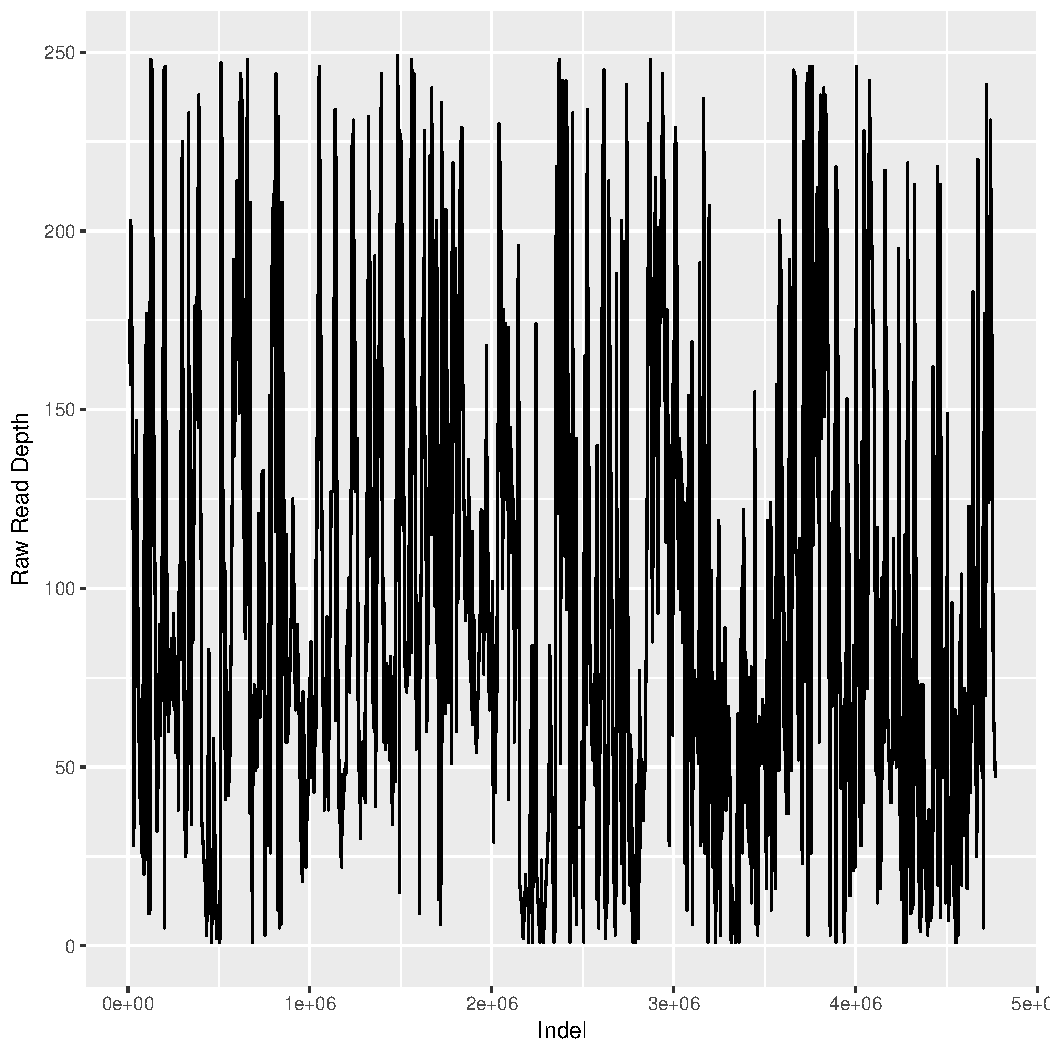
\includegraphics[angle=0,width=1.0\linewidth]{/home/thomas/Directed_Studies_Summer_2019/Armillaria_gallica_gene_analysis_tools/Reporting_documents/Figures/1_DP_locations.pdf}}
		\resizebox{50mm}{50mm}{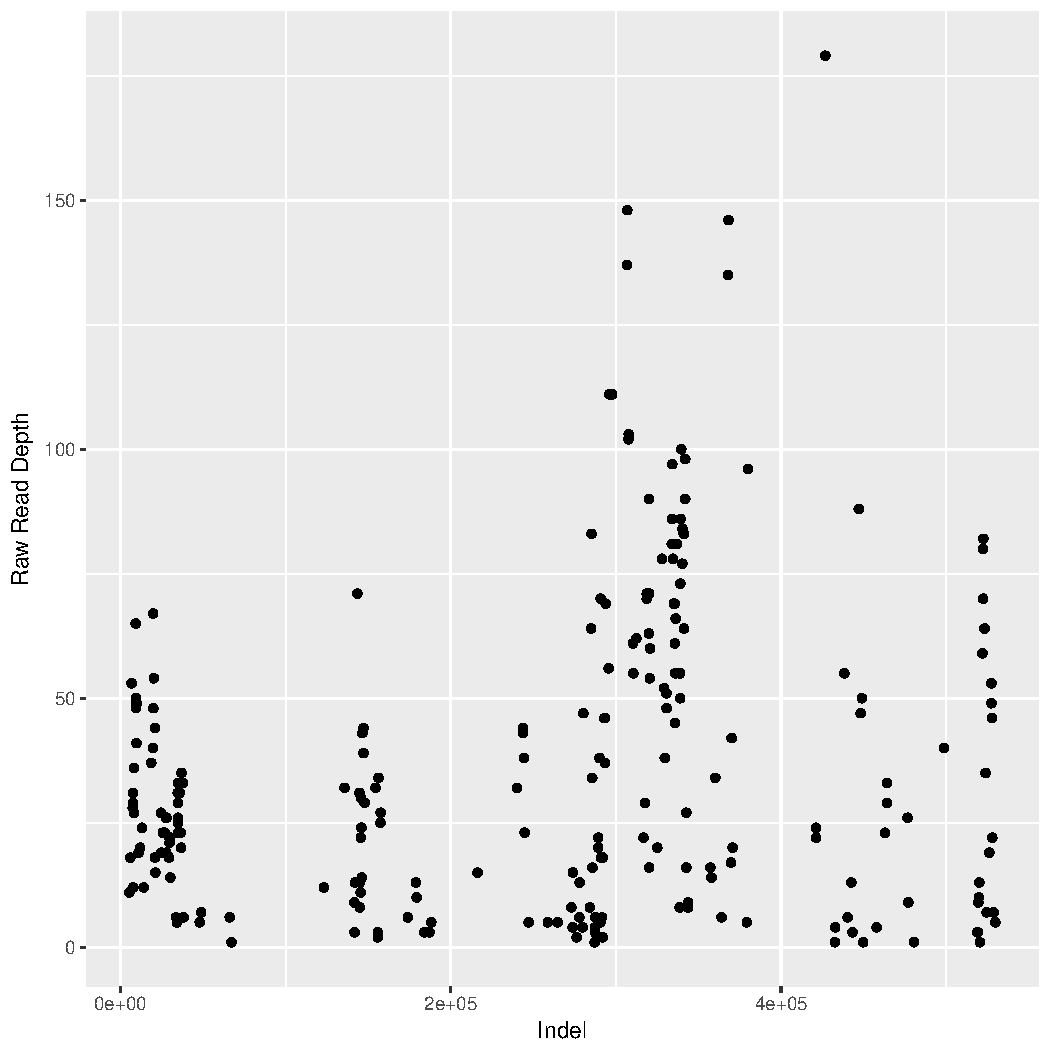
\includegraphics[angle=0,width=1.0\linewidth]{/home/thomas/Directed_Studies_Summer_2019/Armillaria_gallica_gene_analysis_tools/Reporting_documents/Figures/50_DP_locations.pdf}}\\
		\resizebox{50mm}{50mm}{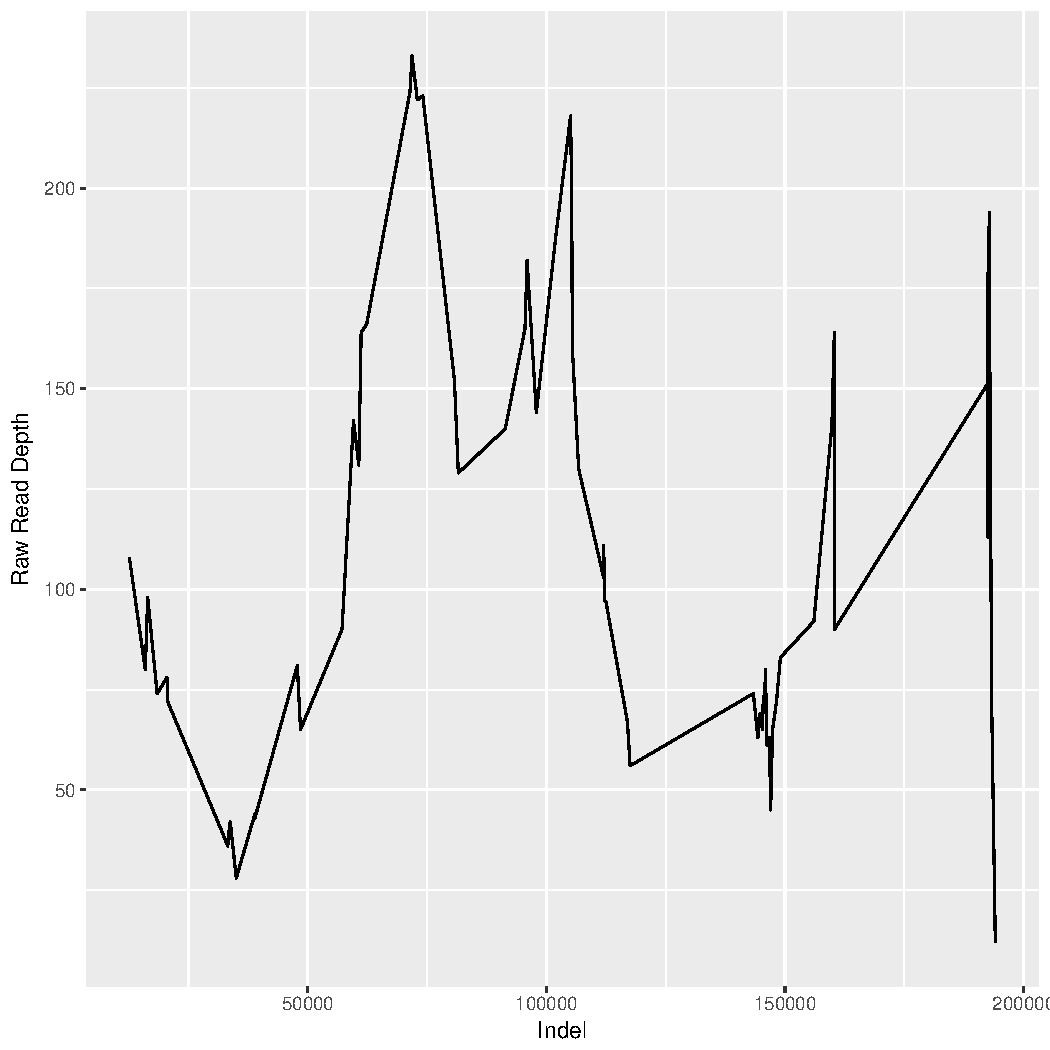
\includegraphics[angle=0,width=1.0\linewidth]{/home/thomas/Directed_Studies_Summer_2019/Armillaria_gallica_gene_analysis_tools/Reporting_documents/Figures/100_DP_locations.pdf}}
		\resizebox{50mm}{50mm}{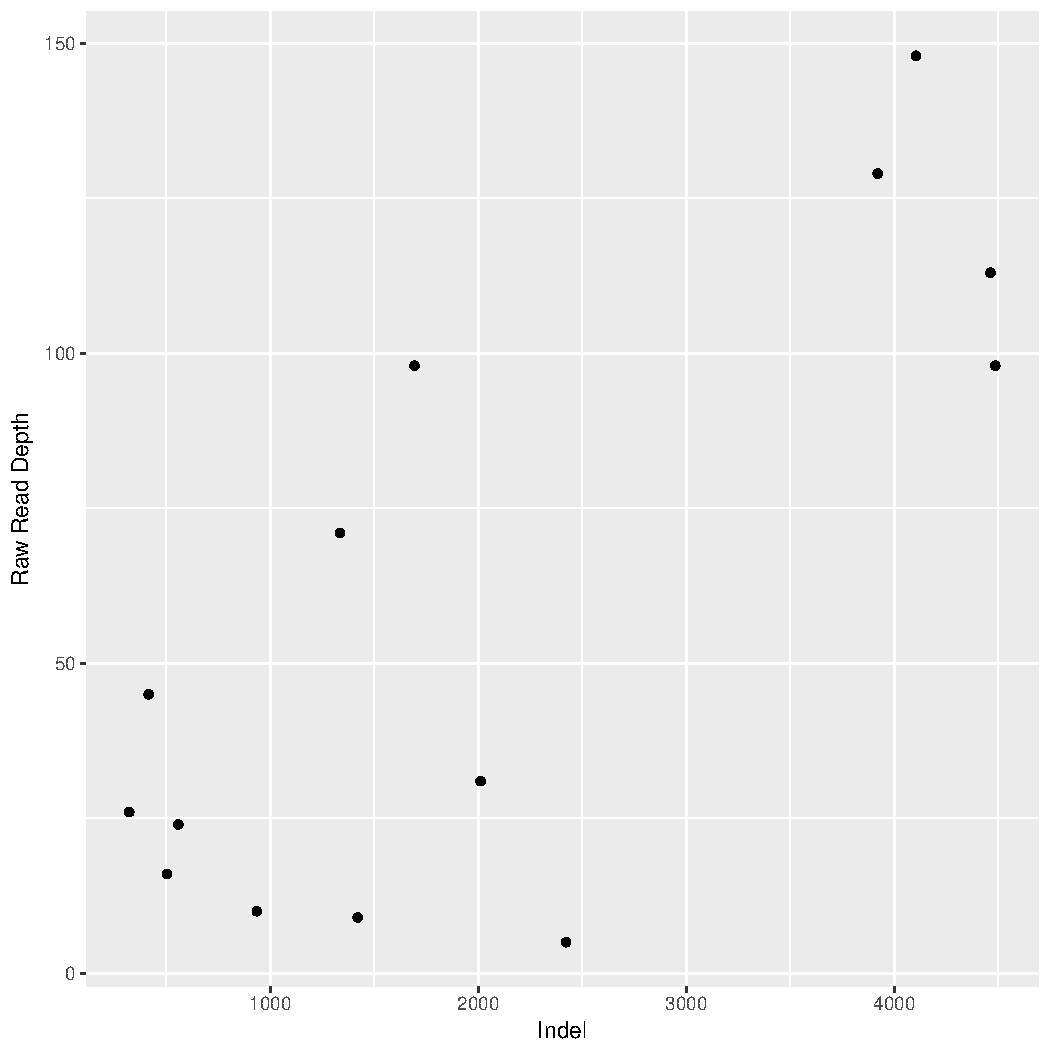
\includegraphics[angle=0,width=1.0\linewidth]{/home/thomas/Directed_Studies_Summer_2019/Armillaria_gallica_gene_analysis_tools/Reporting_documents/Figures/211_DP_locations.pdf}}
		\begin{singlespace}
			\vspace{-0.5cm}
			\caption[The Read Depth of Indels Found]{The Read Depth of Indels Found in Ar109 at scaffold 1, 50, 100 and 211. Every datapoint indicates one indel}\label{readdepth_indel}
		\end{singlespace}
	\end{centering}
\end{figure}

\subsection{Indel Lengths}  

Since given the read depths, it was shown that it would be appropriate to move forward. The next step we did was analyze the difference lengths of indels. This was done by using a very simple command from the package vcftools, the command was \textit{--hist-indel-len}. This gave a very crude histogram as well as the counts for each indel at each length. From this data we created a better visualization of the data. 

It can be seen that the smaller the indel, the more frequent it occurs. This holds true throughout the strains that were tested.

\begin{figure}[H]
	\begin{centering}
		%\vspace{-1.5cm}
		\resizebox{60mm}{60mm}{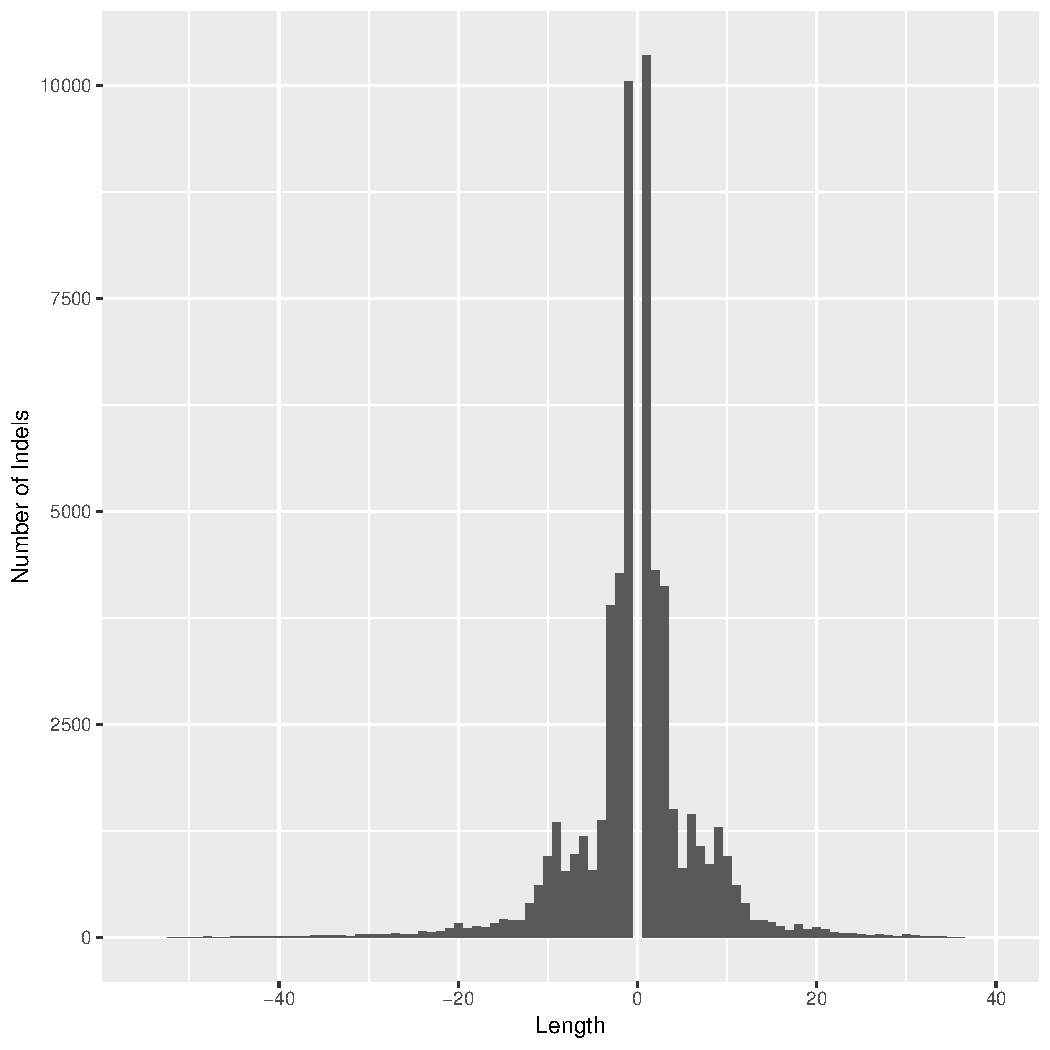
\includegraphics[angle=0,width=0.75\linewidth]{/home/thomas/Directed_Studies_Summer_2019/Armillaria_gallica_gene_analysis_tools/Reporting_documents/Figures/Ar109_histogram.pdf}}
		\resizebox{60mm}{60mm}{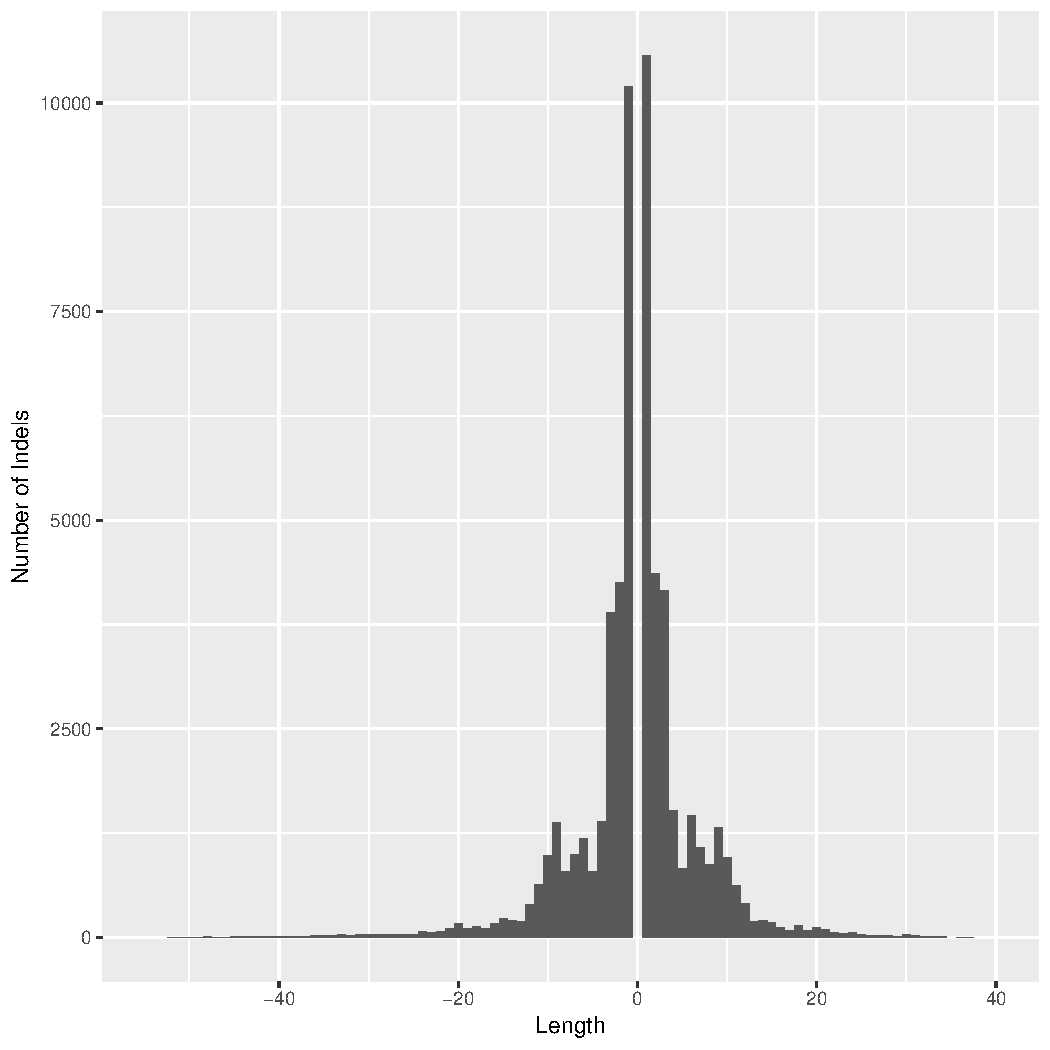
\includegraphics[angle=0,width=0.75\linewidth]{/home/thomas/Directed_Studies_Summer_2019/Armillaria_gallica_gene_analysis_tools/Reporting_documents/Figures/Ar119_histogram.pdf}}\\
		\begin{singlespace}
			\vspace{-0.5cm}
			\caption[The Frequency of the Indel Length]{The Frequency of the Indel Length Per Strain, Ar109 and Ar119}\label{Length_Indel_His}
		\end{singlespace}
	\end{centering}
\end{figure}
 
 
In the histograms, it can be seen that the largest indels were found to be single nucleotide bases. It was a bell-shaped or a normal distribution, which is what to be expected. From this, we focused on the extremities of indels. We explored on the largest insertions detected. We extracted the sequences and the 5 nucleotides that flanked each end, and BLAST-ed these against the NCBI database.  

Many of the BLAST searches came back as empty however, there were a couple of hits throughout the data. We also found many repeated elements within the indel analysis. One BLAST hit that was further looked into was at position 117162 at scaffold 98. It was 44 nucleotides long, which still is not that large in the grand scheme of indels. However, it was a perfect match against \textit{Streptomyces actuosus}. This indel was found in 8 of the 15 strains that were tested. Using the literature, we indicated where this indel was found on the spatial map as well as the phylogeny.
 
 
\begin{figure}[H]
	\begin{centering}
		%\vspace{1.5cm}
		\resizebox{70mm}{70mm}{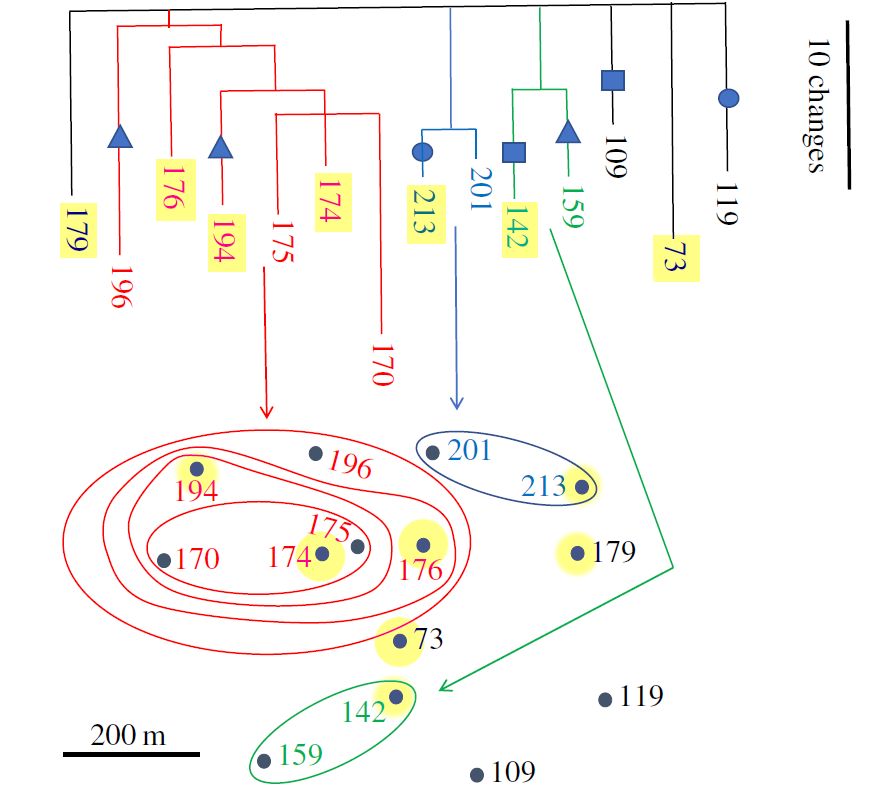
\includegraphics[angle=0,width=1.0\linewidth]{/home/thomas/Directed_Studies_Summer_2019/Armillaria_gallica_gene_analysis_tools/Reporting_documents/Figures/tree_dd.png}}
		\begin{singlespace}
			\vspace{-0.5cm}
			\caption[Phylogeny overlap with \textit{Streptomyces} Indels]{The phylogeny found within the original publication (Anderson \textit{et al}, 2018) with the indication of where the \textit{Steptomyces} Indel was found}\label{tree1}
		\end{singlespace}
	\end{centering}
\end{figure}

\begin{figure}[H]
	\begin{centering}
		%\vspace{1.5cm}
		\resizebox{70mm}{70mm}{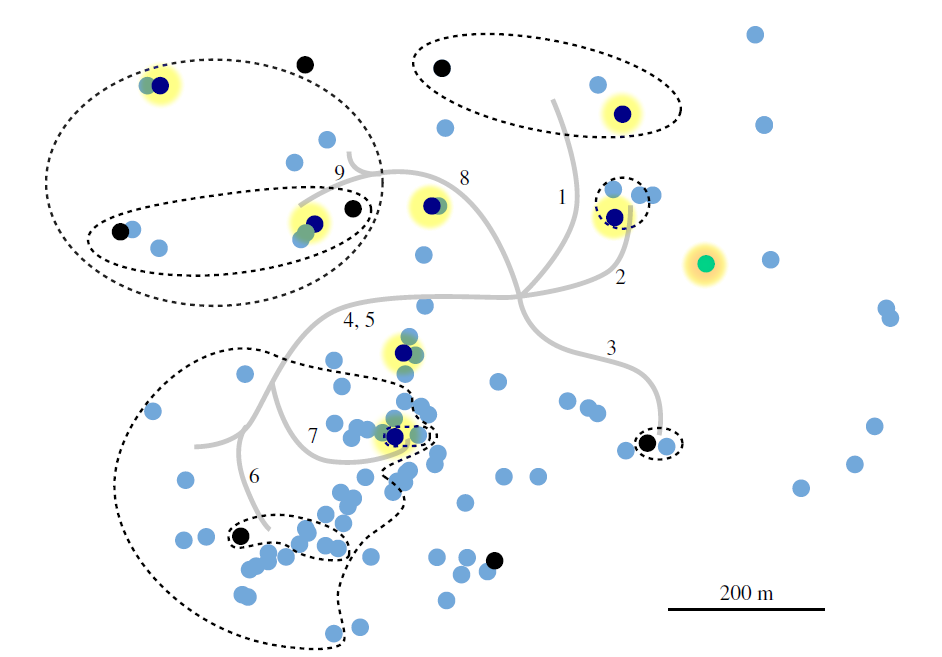
\includegraphics[angle=0,width=1.0\linewidth]{/home/thomas/Directed_Studies_Summer_2019/Armillaria_gallica_gene_analysis_tools/Reporting_documents/Figures/tree_dd2.png}}
		\begin{singlespace}
			\vspace{-0.5cm}
			\caption[Spatial map overlap with \textit{Streptomyces} Indels]{The spatial map found within the original publication (Anderson \textit{et al}, 2018) with the indication of where the \textit{Steptomyces} Indel was found}\label{tree2}
		\end{singlespace}
	\end{centering}
\end{figure}

In order to show a better representation, we included the actual sequence of the found indel and the flanking regions around it. In the sequences where the indel is not present, the sequence would be linear.


\begin{figure}[H]
	\begin{centering}
		\vspace{1.5cm}
		\resizebox{150mm}{50mm}{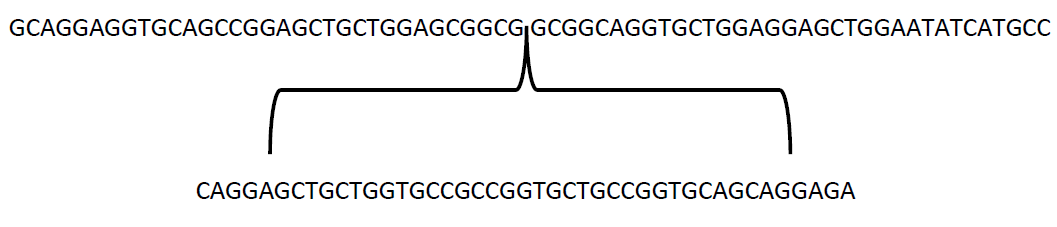
\includegraphics[angle=0,width=1.0\linewidth]{/home/thomas/Directed_Studies_Summer_2019/Armillaria_gallica_gene_analysis_tools/Reporting_documents/Figures/177162.png}}
		\begin{singlespace}
			\vspace{-0.5cm}
			\caption[Sequence with \textit{Streptomyces} Indel]{The placement of the found indel in the sequence of the reference genome}\label{seqindel}
		\end{singlespace}
	\end{centering}
\end{figure}


%%%%%%%%%%%%%%%%%%%%%%%%%%%%%%%%%%%
%
%	Future Directions
%
%%%%%%%%%%%%%%%%%%%%%%%%%%%%%%%%%%%
\vspace{-0.5cm}
\section{Future Directions}
\vspace{-0.5cm}
\begin{itemize}
\item Attempt to find larger indels using a different methodology
\vspace{-0.5cm}
\item Take full inventory, via blastn, of all the indels identified and the immediate regions surrounding them 
\vspace{-0.5cm}
\item Create a more robust method to search for regions of high read depth
\vspace{-0.5cm}
\item Take full inventory of all the sequences at regions of high read depth
\vspace{-0.5cm}
\item Look at the sequences which result from comparison of 
\vspace{-0.5cm}
\item Search for transposons
\vspace{-0.5cm}
\item Complete De novo assemblies and carry out many of these analyses on those
\vspace{-0.5cm}
\item Look into the reads which did not align to the reference and attempt to find any variation which may exist between the strains
\end{itemize}

\end{document}



